\chapter{Implementasi dan Evaluasi}

Bab ini membahas hasil implementasi dari rancangan solusi pada Bab
\ref{chapter-3}. Bab ini juga membahas validasi hasil implementasi untuk
memastikan bahwa hasil implementasi mencapai tujuan validasi. Selain itu, Bab
ini membahas mengenai distribusi hasil implementasi dan evaluasi.

\section{Hasil Eksplorasi CARLA}

Setelah membaca dokumentasi CARLA, menginstal CARLA (CARLA, CARLAUE4, dan editor
CARLAUE4), dan mengeksplorasi editor CARLAUE4 diketahui terdapat beberapa fitur
sebagai berikut:

\begin{enumerate}
    \item Penambahan kendaraan baru beroda empat dan dua
    \item Penambahan objek \textit{spline} untuk menambahkan rel
    \item Penambahan objek statis lainnya
\end{enumerate}

% note: ? tambah hasil eksplorasi lainnya (eksplorasi buat kota baru)

\section{Implementasi}

Bagian ini membahas mengenai batasan implementasi, implementasi trem dan angkot
sebagai kendaraan roda 4, sepeda onthel, sepeda motor, dan becak sebagai
kendaraan roda 2, stasiun dan rambu lalu lintas sebagai objek statis, dan rel
sebagai objek statis dalam bentuk \textit{spline}.

\subsection{Batasan Implementasi}

Objek lokal dan lingkungan dibuat menggunakan Blender versi 3.3 LTS dan
diimplementasikan menggunakan CARLA versi 0.9.12 pada sistem operasi Linux
Ubuntu 18.04 LTS dan CARLA versi 0.9.13 pada sistem operasi Windows 11.
Implementasi dilakukan pada dua sistem operasi yang berbeda agar memermudah
proses implementasi karena CARLA di komputer dengan sistem operasi Ubuntu
digunakan bersama untuk SILS dan CARLA di komputer dengan sistem operasi Windows
adalah komputer pribadi. Hasil implementasi hanya didistribusikan untuk sistem
operasi Linux (Ubuntu). Implementasi objek lokal dan lingkungan yang dilakukan
adalah sebagai berikut:

\begin{enumerate}
    \item Trem dan angkot sebagai kendaraan roda 4
    \item Sepeda onthel, sepeda motor, dan becak sebagai kendaraan roda 2
    \item Stasiun Madiun, Stasiun Solokota, dan rambu-rambu lalu lintas sebagai
    objek statis
    \item Rel sebagai objek statis dalam bentuk \textit{spline}
\end{enumerate}

% note: https://github.com/carla-simulator/carla/blob/0.9.13/CHANGELOG.md

\subsection{Implementasi Trem dan Angkot}

Implementasi trem dan angkot sebagai kendaraan roda 4 terbagi menjadi dua
bagian, yaitu: pembuatan aset model 3D untuk ekspor berkas FBX, dan
pengimporan berkas FBX dan konfigurasi kendaraan roda 4 dalam editor CARLAUE4.

\subsubsection{Pembuatan Aset Model 3D untuk Ekspor Berkas FBX}

Implementasi trem dan angkot mengikuti langkah-langkah pada
\textcite{carla-documentation}. Pembuatan \textit{mesh} model 3D perlu sesuai
dengan persyaratan dari CARLA, yaitu jumlah tris (segitiga satuan yang membentuk
permukaan) berkisar antara 50.000 hingga 100.000 dan melakukan pemisahan
material atau tekstur sesuai dengan bagian kendaraan agar tampilan sesuai saat
disimulasikan. Ukuran model 3D disesuaikan dengan ukuran yang asli karena hasil
impor menggunakan rasio 1 banding 1.

Setelah model 3D dibuat, aset \textit{vehicle skeleton} atau \textit{armature}
dari \textcite{carla-documentation} ditambahkan, diatur posisi \textit{bone}
dari \textit{armature}, dan dihubungkan ke \textit{mesh} model 3D. Gambar
\ref{fig:vehicle-skeleton} menunjukkan aset yang harus ditambahkan pada
kendaraan. Setelah \textit{armature} ditambahkan, masing-masing \textit{head}
dari \textit{bone} roda perlu diposisikan di tengah ban. Gambar
\ref{fig:armature-placement} menunjukkan penempatan \textit{armature}. Aset
\textit{armature} hanya boleh ditranslasi dan tidak boleh dirotasi ataupun
diatur skalanya karena akan merusak proses impor nantinya.

\begin{figure}[!h]
    \centering
    \subfloat[\textit{Armature}]{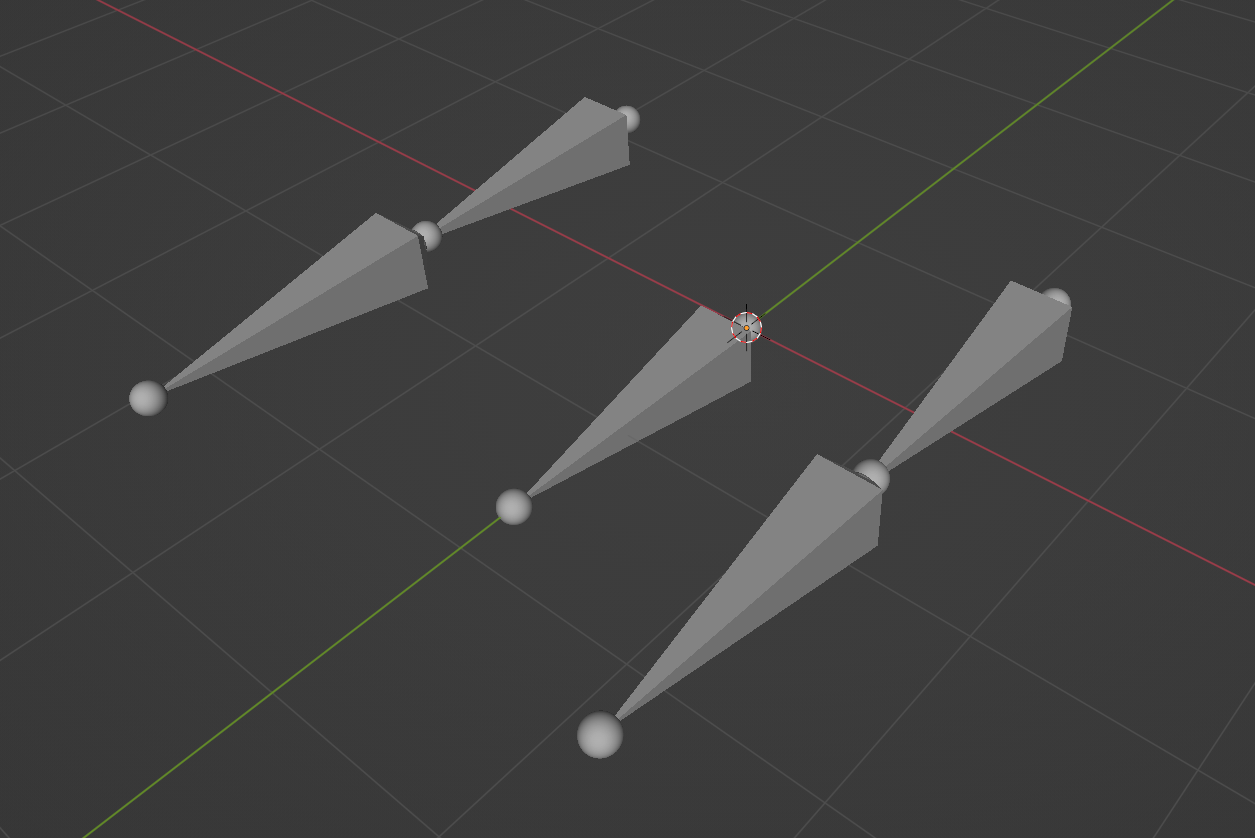
\includegraphics[width=0.4\textwidth]{resources/chapter-4/vehicle-skeleton.png}}
    \hfill
    \subfloat[Hierarki \textit{vehicle skeleton}]{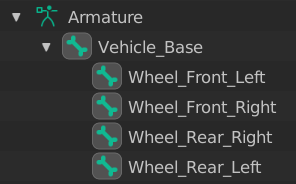
\includegraphics[width=0.4\textwidth]{resources/chapter-4/vehicle-skeleton-hierarchy.png}}
    \caption{\textit{Vehicle skeleton} kendaraan roda 4}
    \label{fig:vehicle-skeleton}
\end{figure}

\begin{figure}[!h]
    \centering
    \subfloat[Tampak depan roda depan kiri angkot]{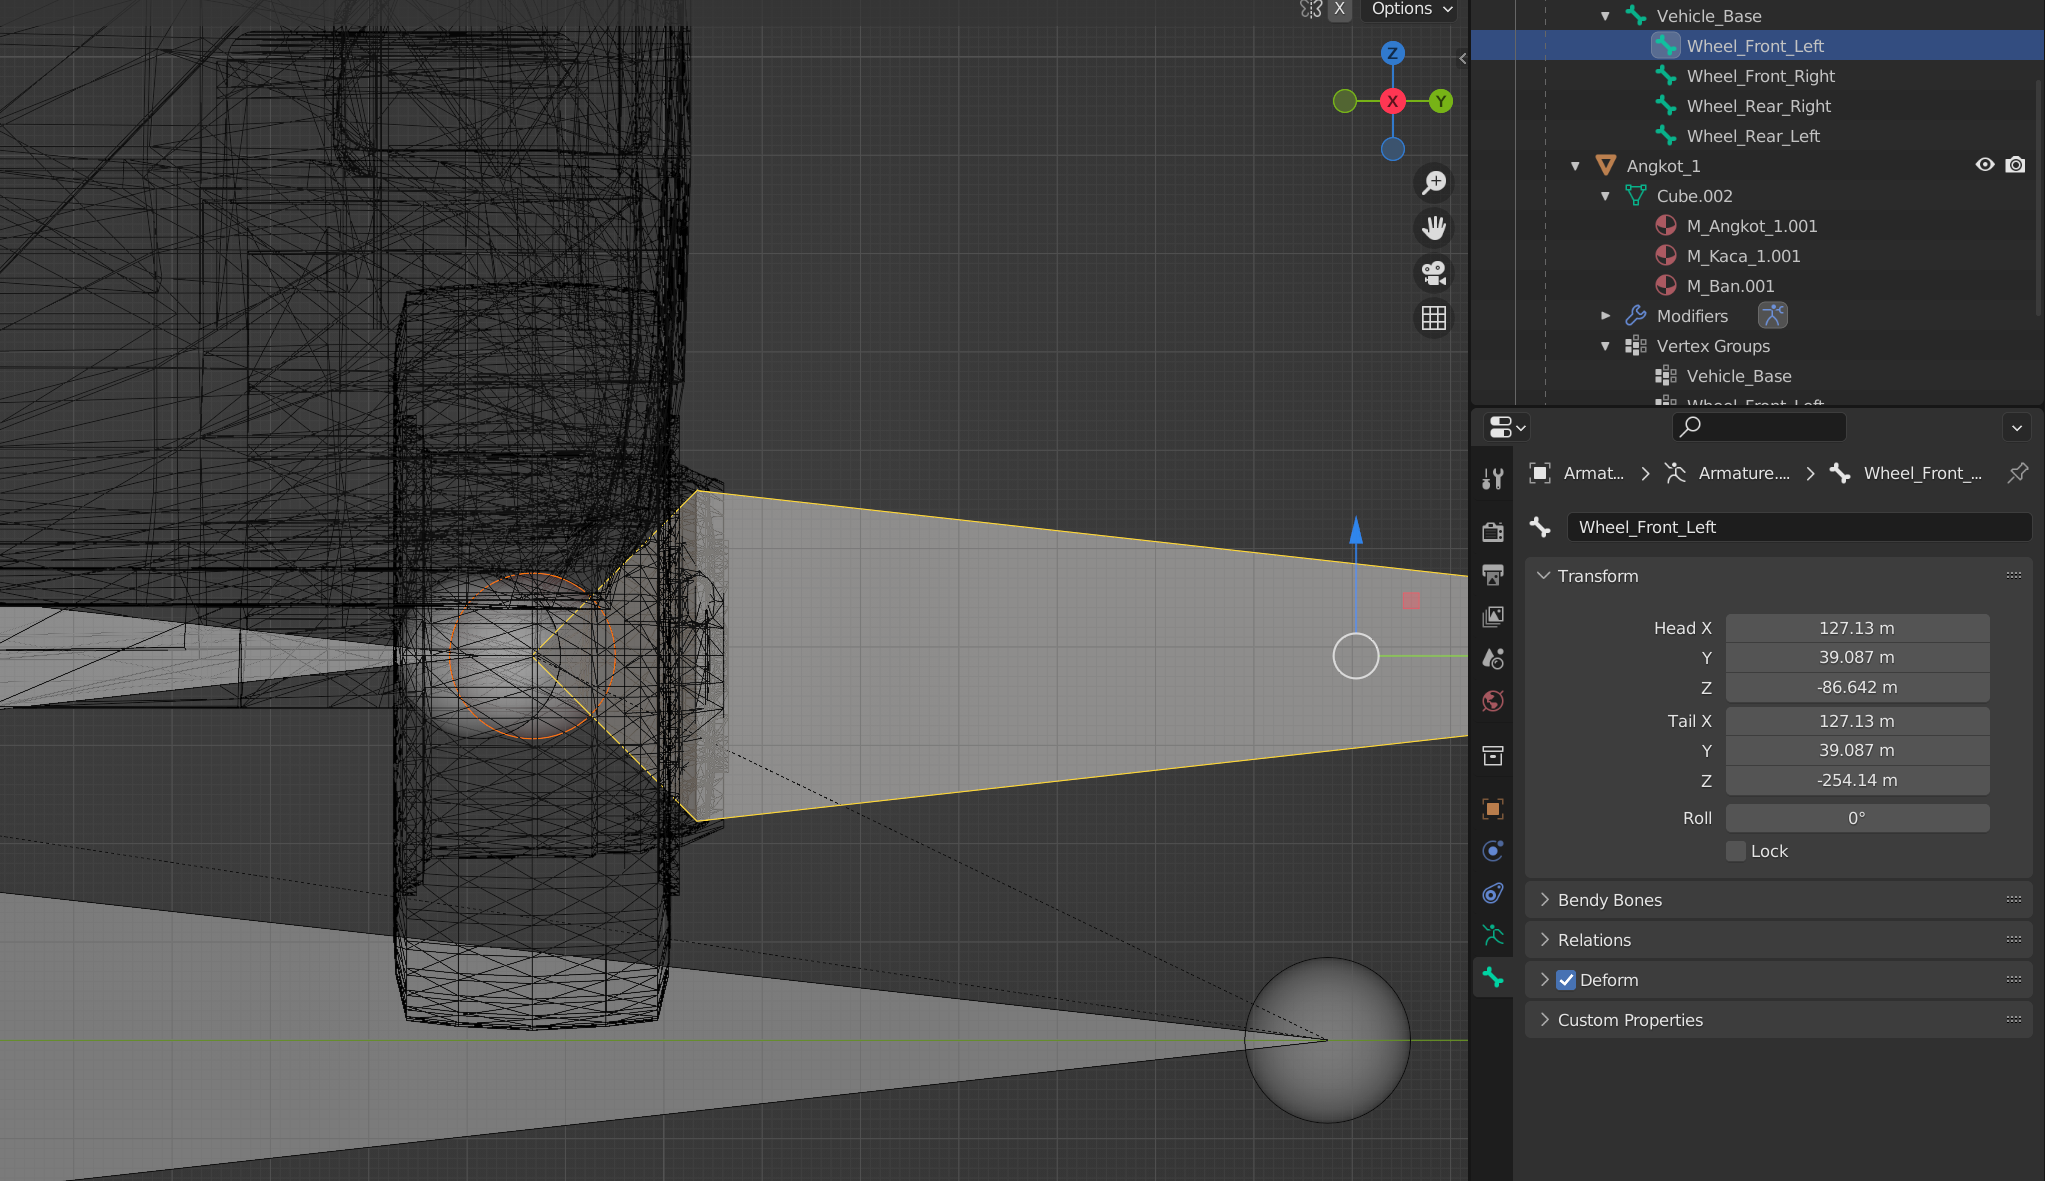
\includegraphics[width=0.45\textwidth]{resources/chapter-4/bone-placement-1.png}}
    \hfill
    \subfloat[Tampak samping roda depan kiri angkot]{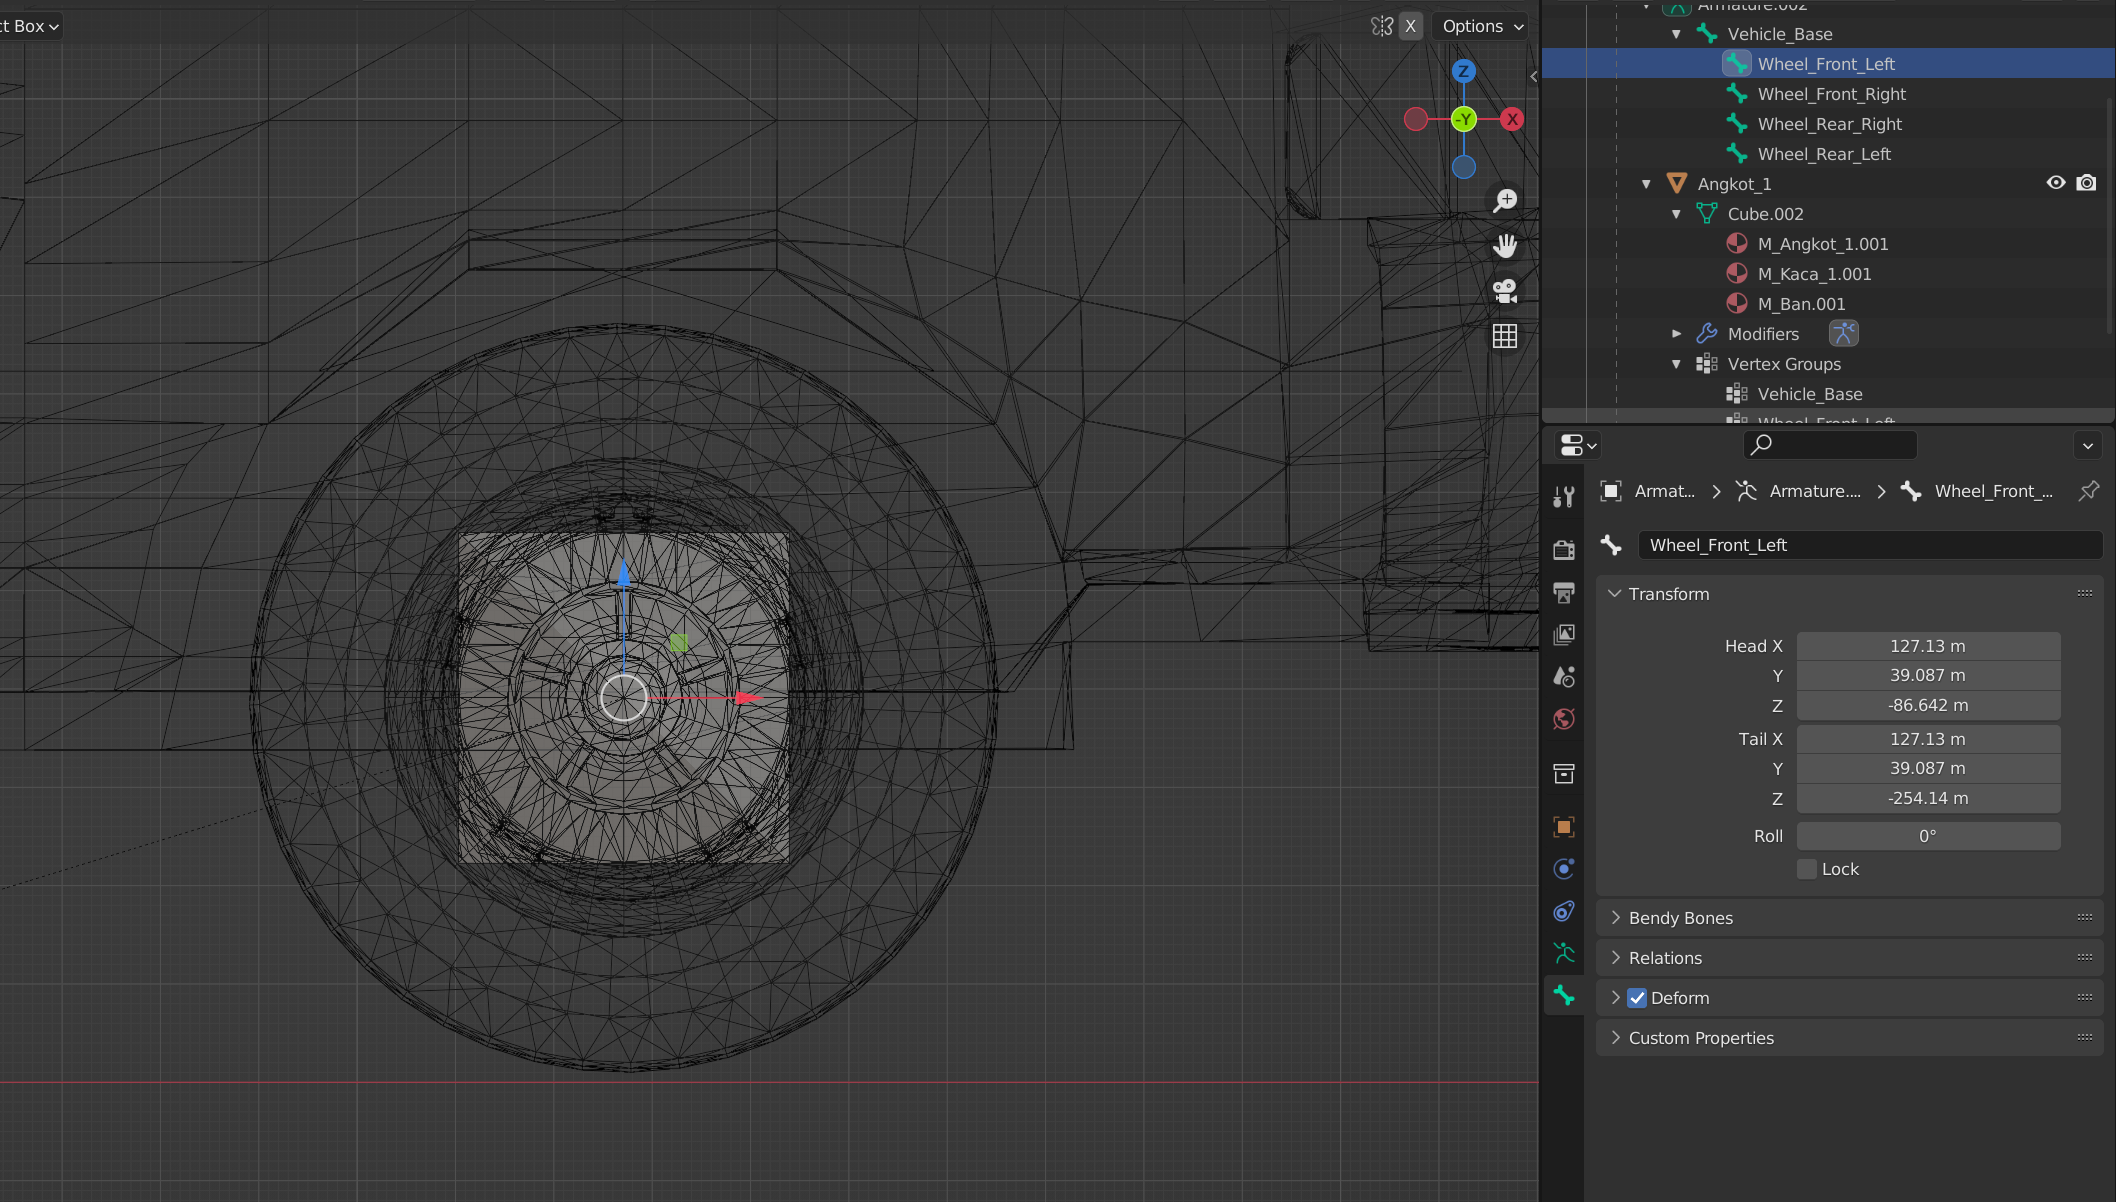
\includegraphics[width=0.45\textwidth]{resources/chapter-4/bone-placement-2.png}}
    \hfill
    \subfloat[Trem dengan \textit{armature} yang telah diatur posisinya]{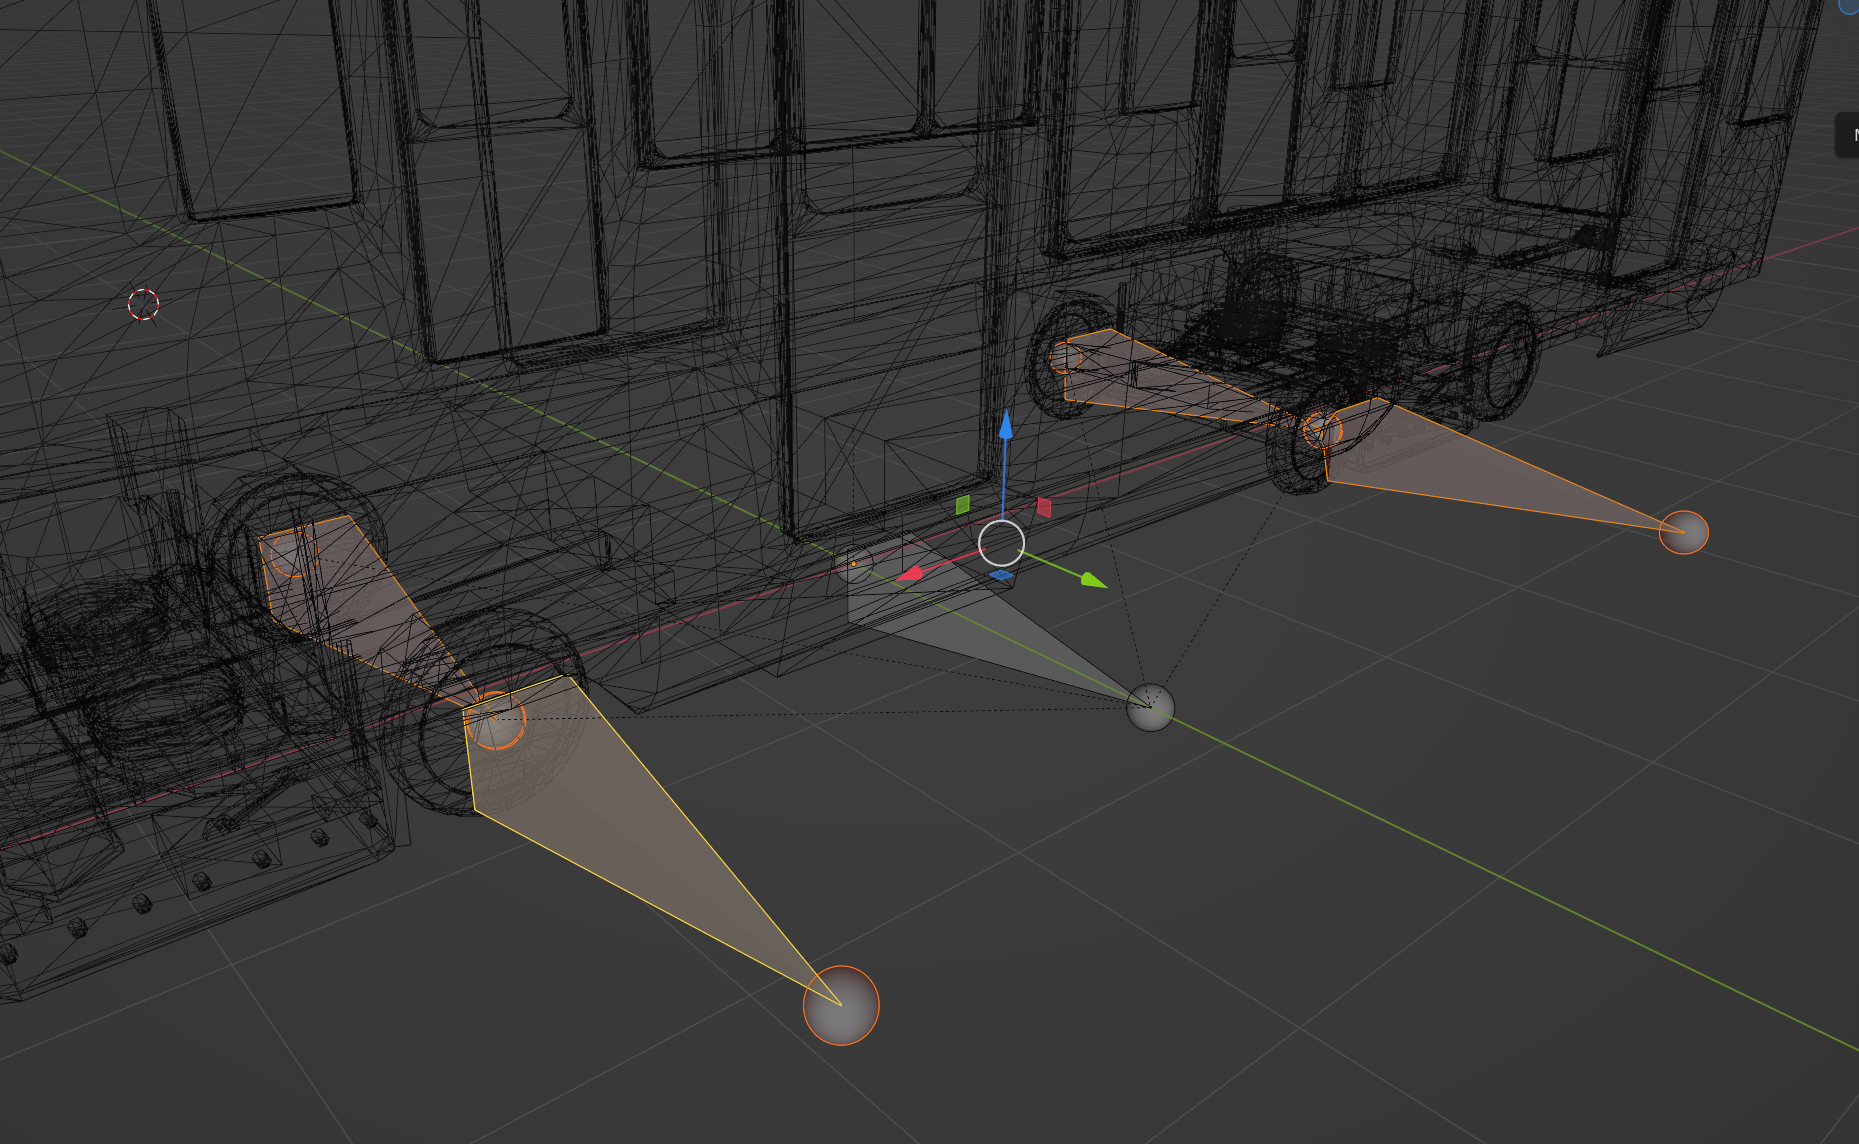
\includegraphics[width=0.45\textwidth]{resources/chapter-4/tram-wheels-bone.png}}
    \caption{Penempatan \textit{armature}}
    \label{fig:armature-placement}
\end{figure}

Setelah semua posisi \textit{bone} sesuai, dilakukan \textit{skinning} antara
\textit{armature} dengan \textit{mesh} kendaraan. Lima \textit{vertices groups}
dibuat untuk menghubungkan kumpulan titik dengan \textit{bone} yang sesuai.
Kelima \textit{vertices groups} dibuat dengan nama yang sesuai dengan nama
\textit{bone} yang akan dihubungkan. Gambar \ref{fig:vertices-groups}
menunjukkan \textit{vertices groups} yang sudah dibuat dan ditambahkan kumpulan
titiknya. \textit{Vertices groups} dibuat dengan cara memasuki \textit{edit
mode} (pada mesh kendaraan) dan menambahkan \textit{vertices groups} pada
\textit{tab} \verb|Object Data Properties|. Setelah itu, \textit{vertices
groups} tersebut diisi dengan titik-titik yang sesuai.

\begin{figure}[!h]
    \centering
    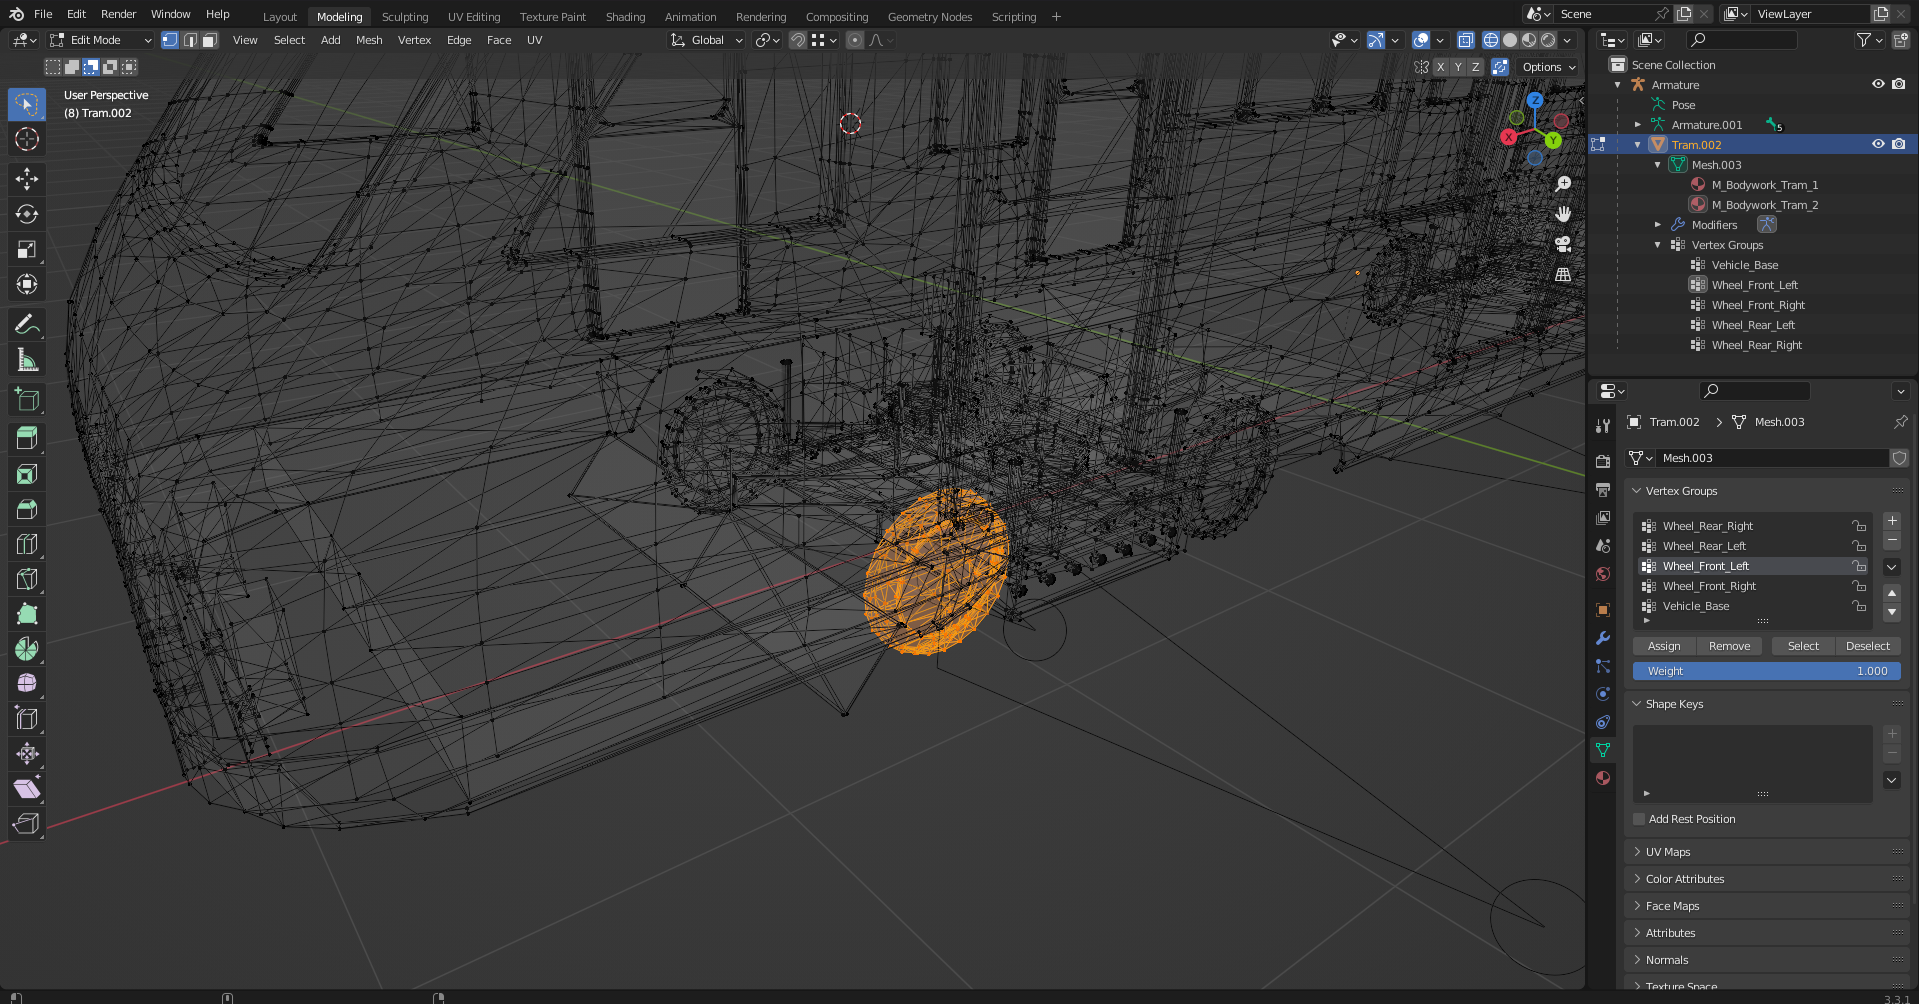
\includegraphics[width=1\textwidth]{resources/chapter-4/vertices-groups.png}
    \caption{\textit{Vertices groups} yang telah dibuat}
    \label{fig:vertices-groups}
\end{figure}

Dilakukan \textit{skinning} dengan cara memasuki \textit{object mode} dan
menyusun hierarki objek seperti pada Gambar \ref{fig:skinning-hierarchy}
kemudian memilih menu \verb|Object > Parent > Armature Deform with Automatic|
yang terletak pada \textit{Viewport Header}. Gambar \ref{fig:wheel-skinning}
menunjukkan roda angkot bagian depan kiri yang sudah dihubungkan dengan
\textit{bone} yang sesuai. Pengujian ini dilakukan dengan memilih salah satu
\textit{bone}, mengetik `r', dan menggerakkan \textit{cursor} pada \textit{pose
mode}.

\begin{figure}[!h]
    \centering
    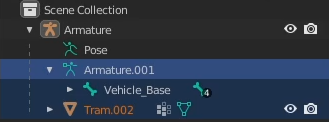
\includegraphics[width=0.6\textwidth]{resources/chapter-4/skinning-hierarchy.png}
    \caption{Hierarki objek}
    \label{fig:skinning-hierarchy}
\end{figure}

\begin{figure}[!h]
    \centering
    \subfloat[Roda posisi awal]{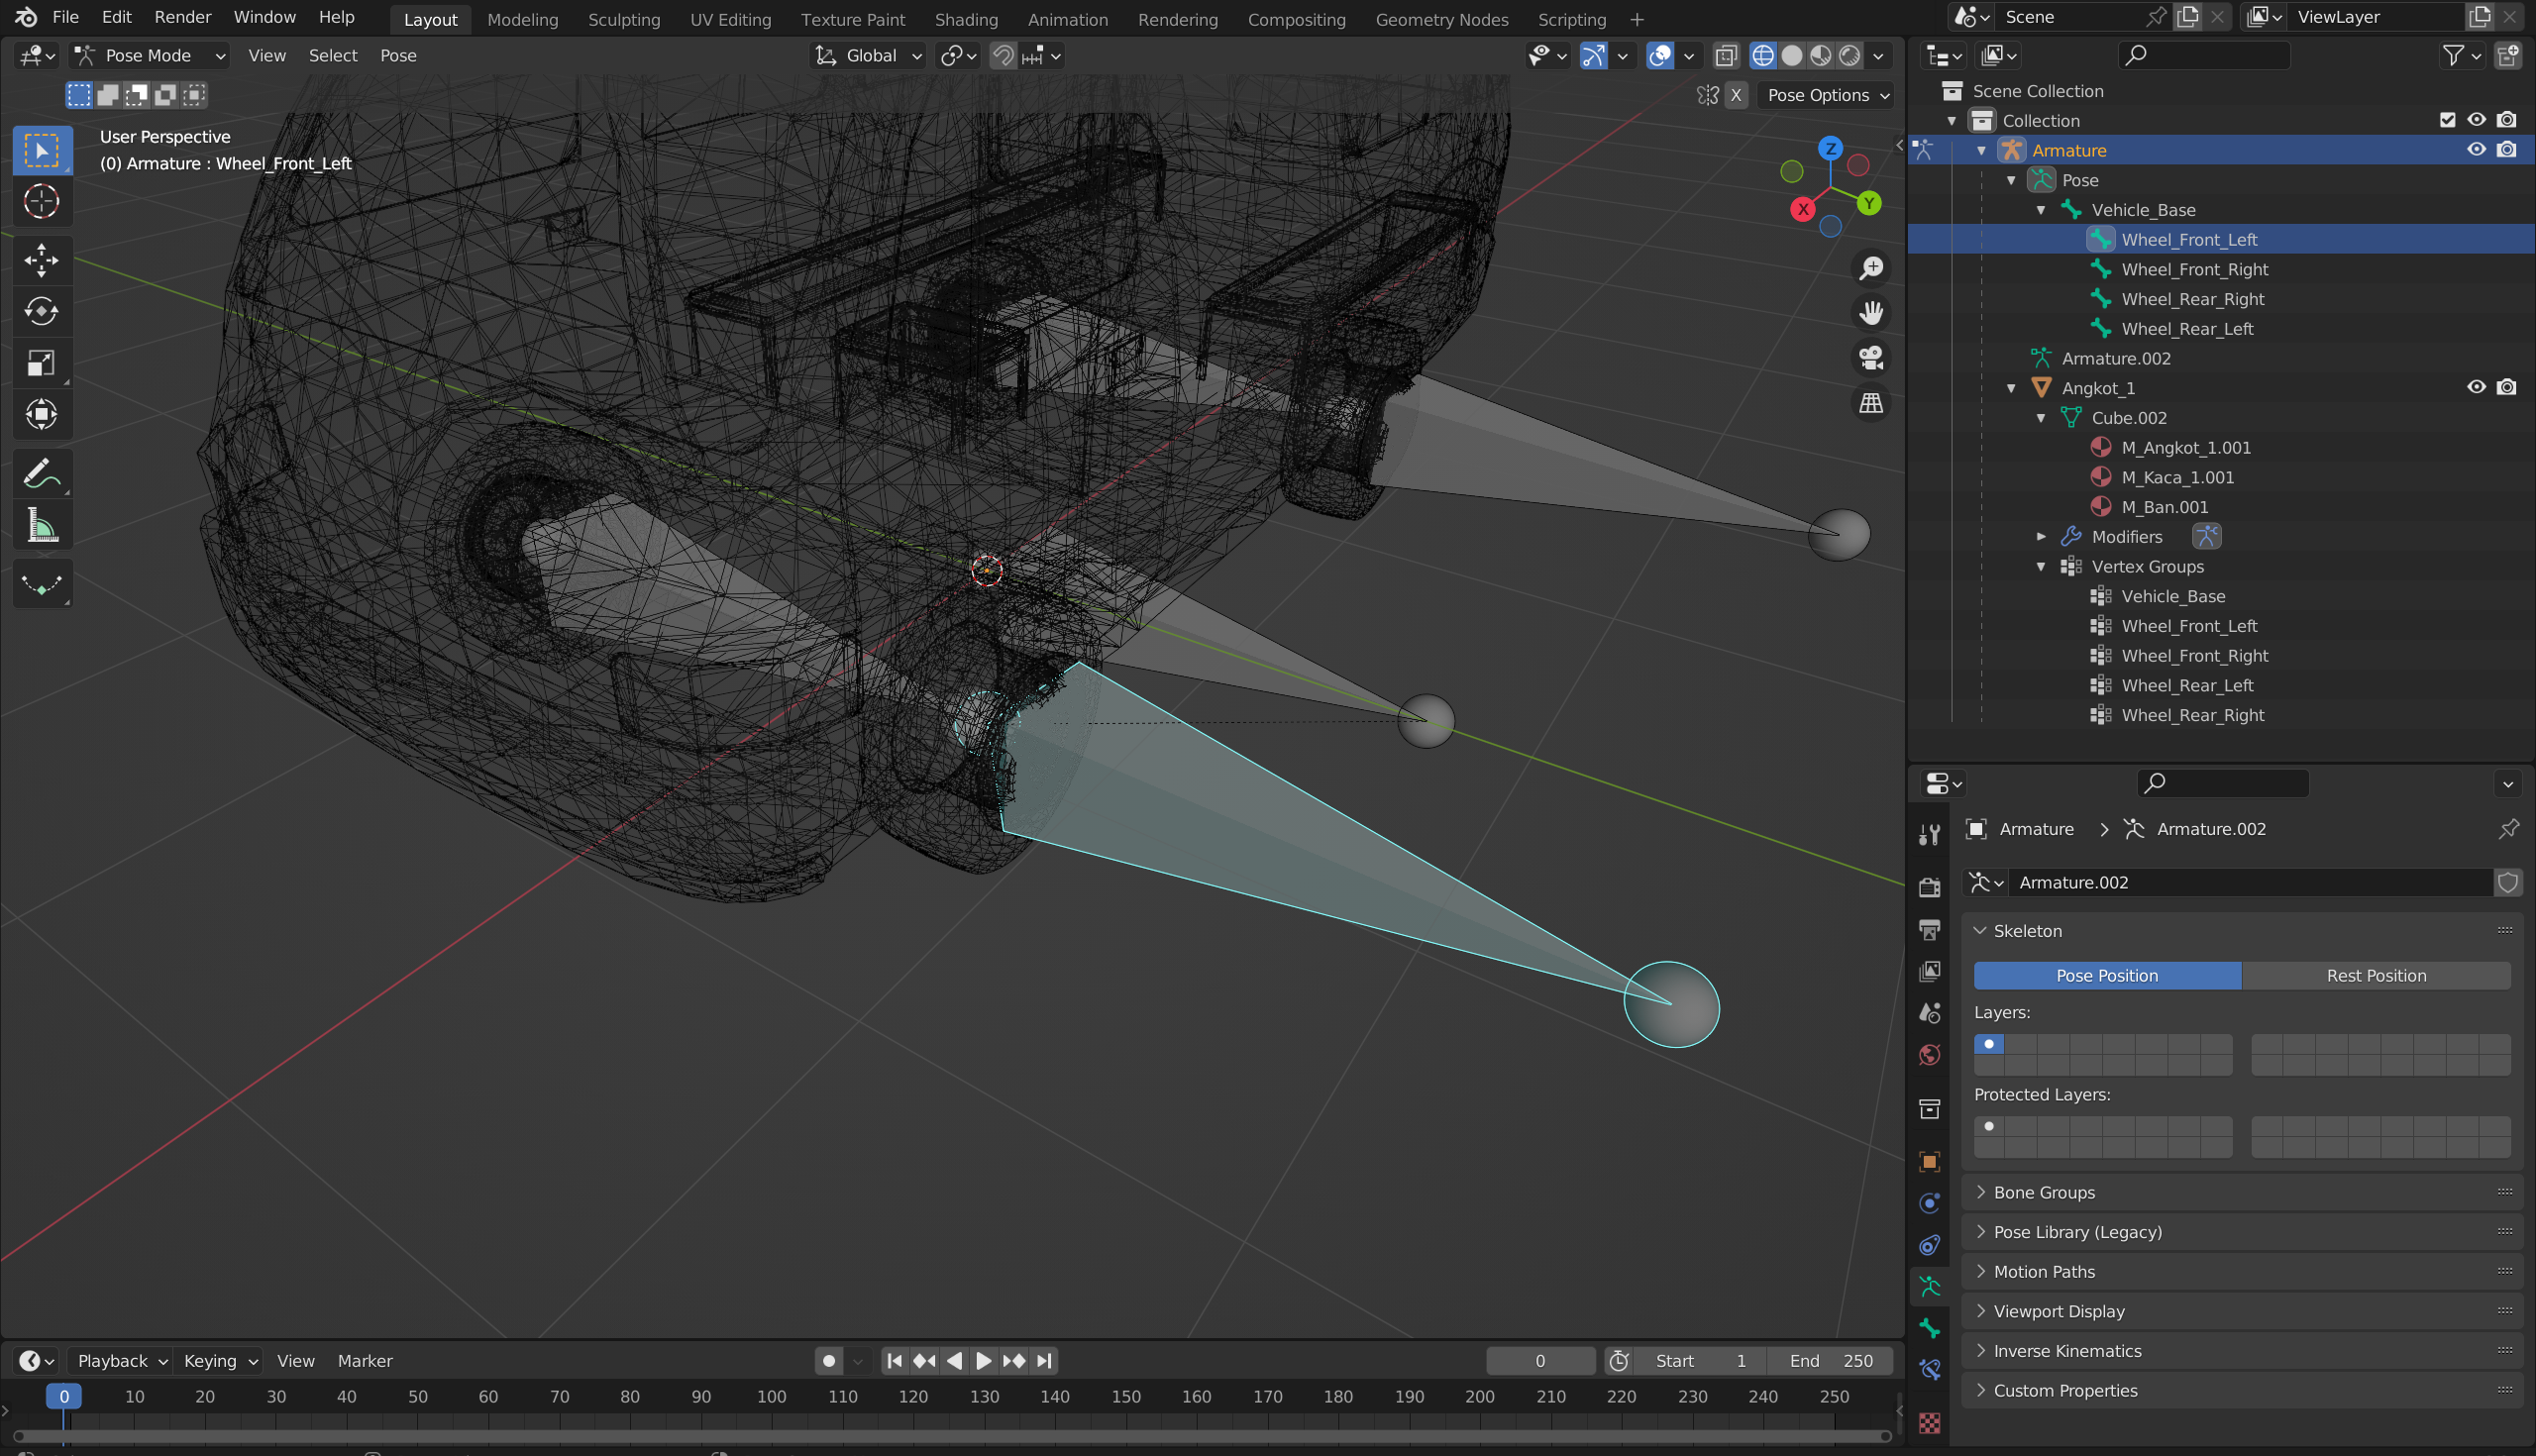
\includegraphics[width=0.47\textwidth]{resources/chapter-4/skinned-wheel-default.png}}
    \hfill
    \subfloat[Perubahan posisi roda]{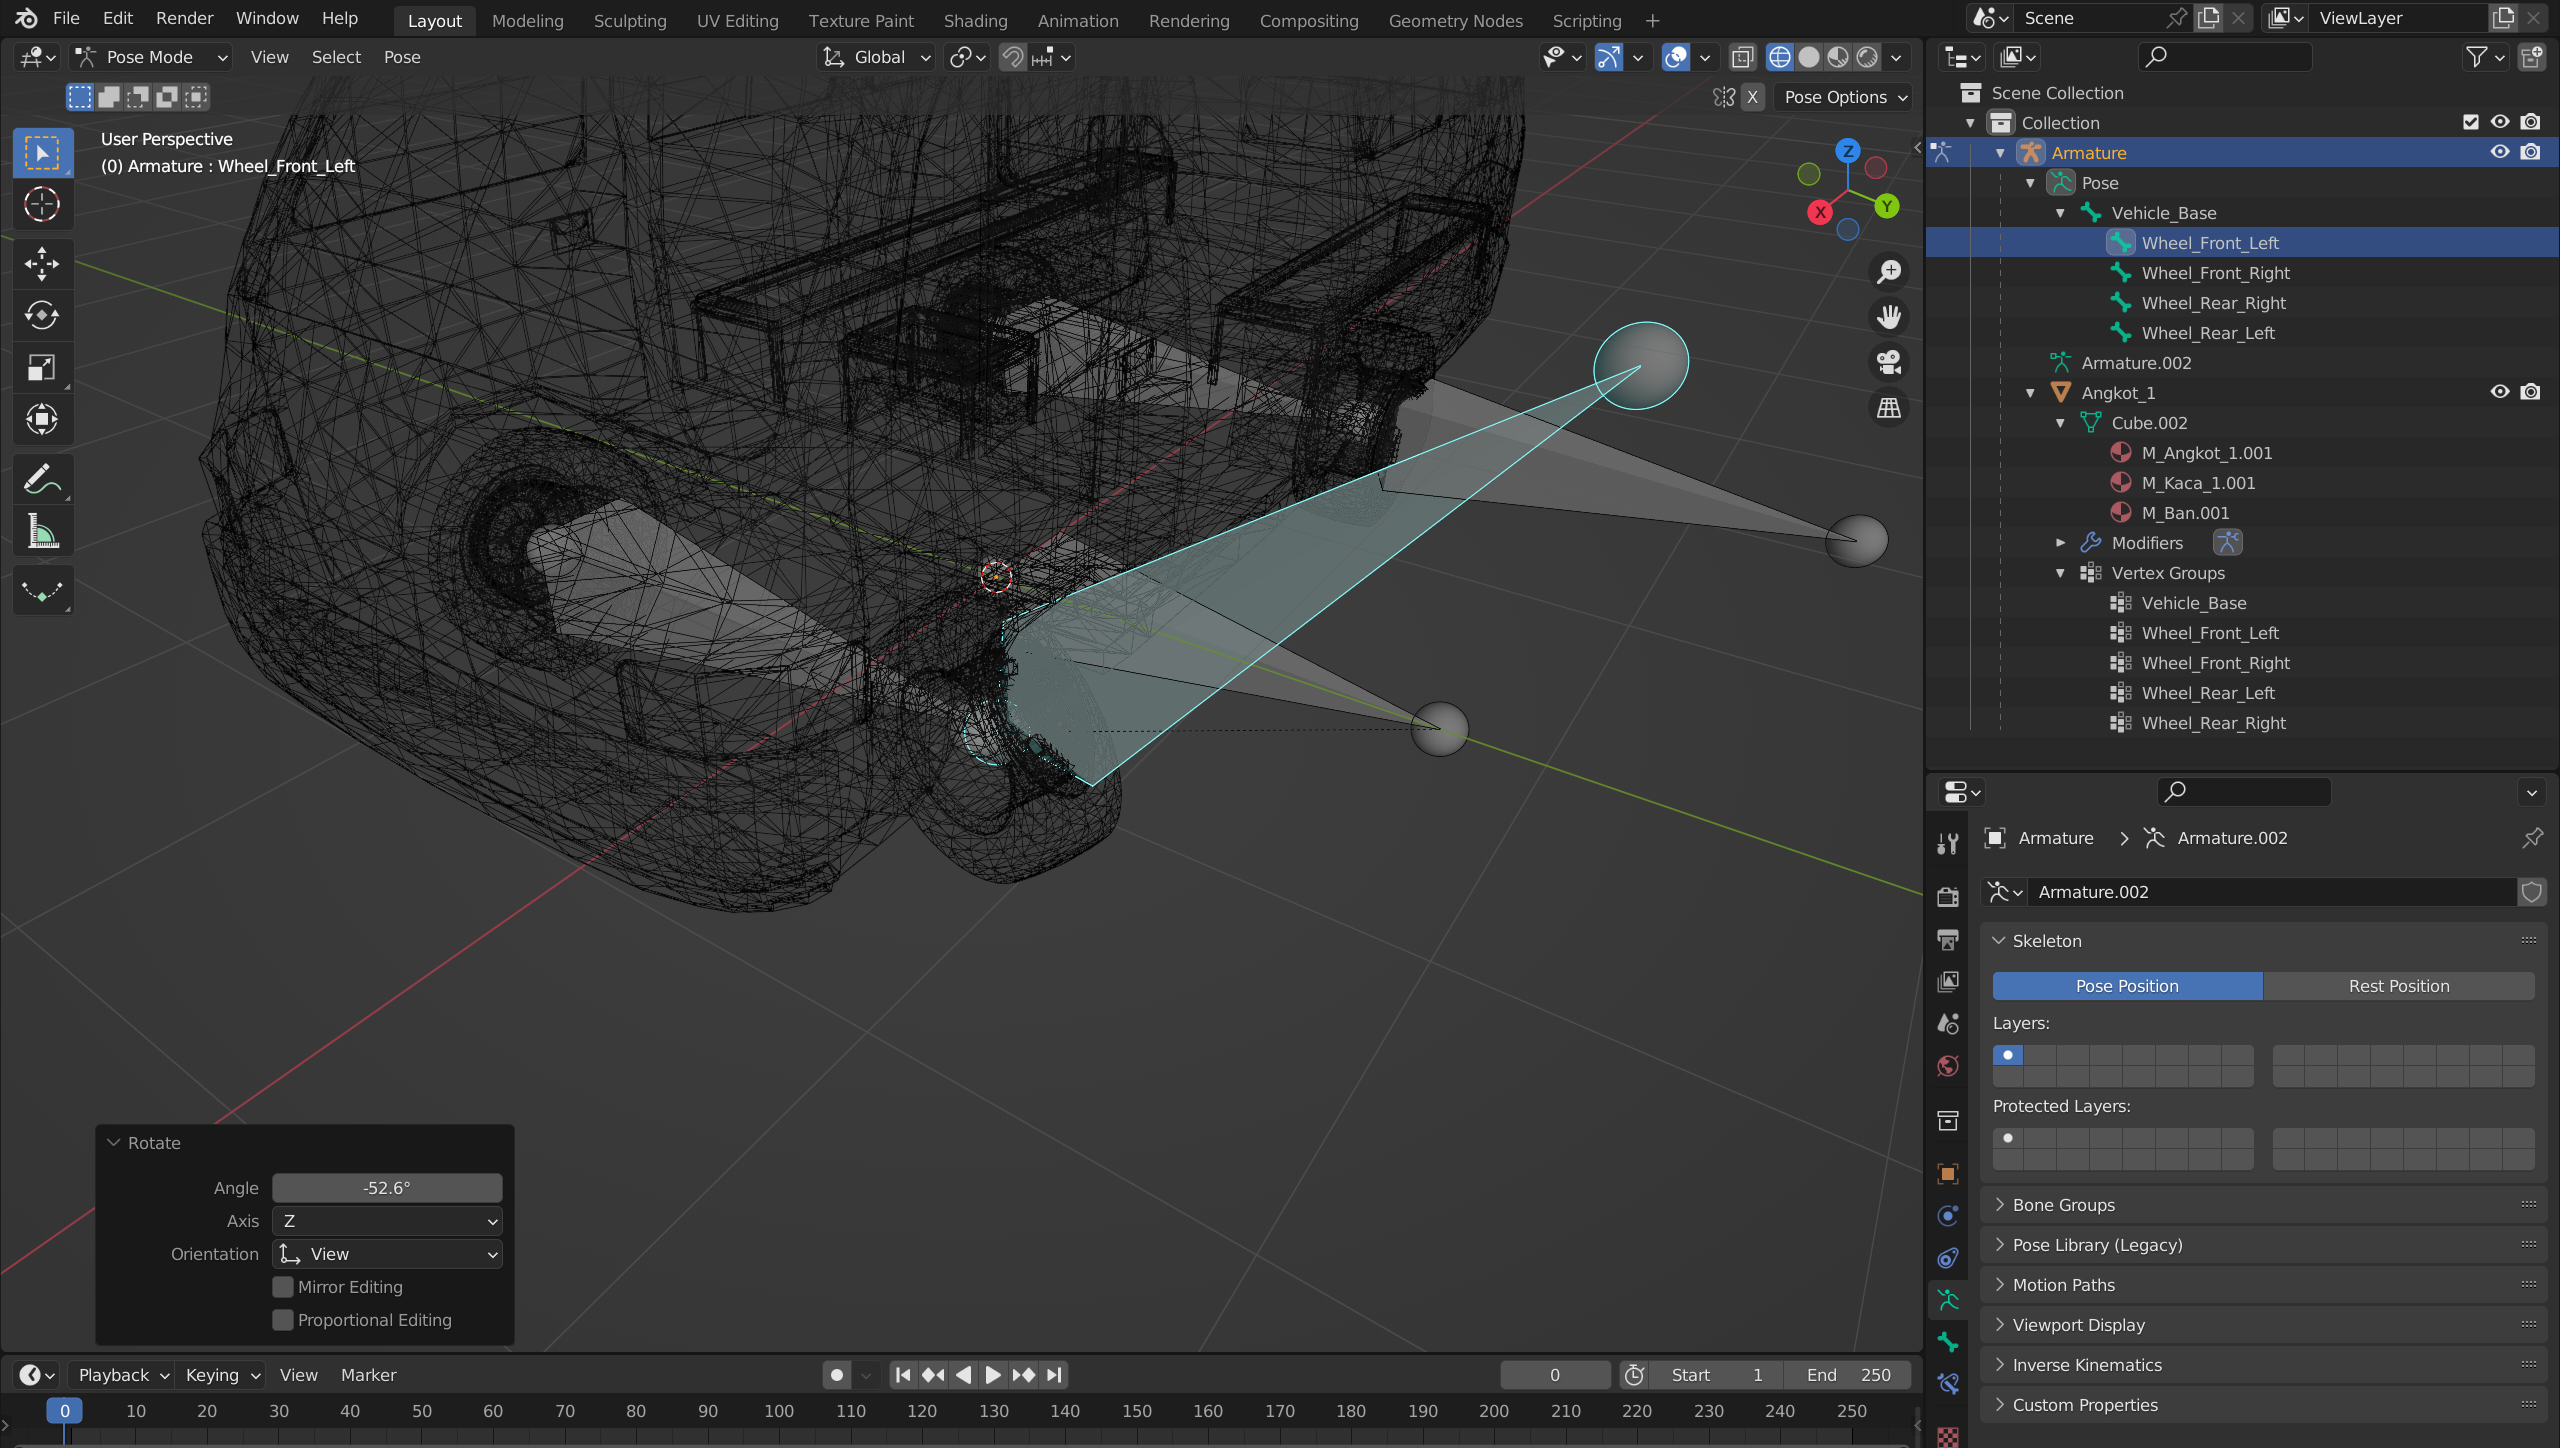
\includegraphics[width=0.47\textwidth]{resources/chapter-4/skinned-wheel-moved.png}}
    \caption{Hasil \textit{skinning} roda yang benar}
    \label{fig:wheel-skinning}
\end{figure}

Aset model 3D kemudian diekspor ke dalam format FBX. Gambar \ref{fig:export-fbx}
menunjukkan opsi ekspor yang digunakan. Opsi yang perlu diperhatikan adalah opsi
\verb|Forward| dan \verb|Up| pada bagian \verb|Transform|. Opsi \verb|Forward|
diatur ke arah sumbu \verb|-Z Forward| dan opsi \verb|Up| diatur ke arah sumbu
\verb|Y Up|. Opsi lainnya dapat diatur sesuai kebutuhan.

\begin{figure}[!h]
    \centering
    \subfloat[Opsi ekspor berkas FBX]{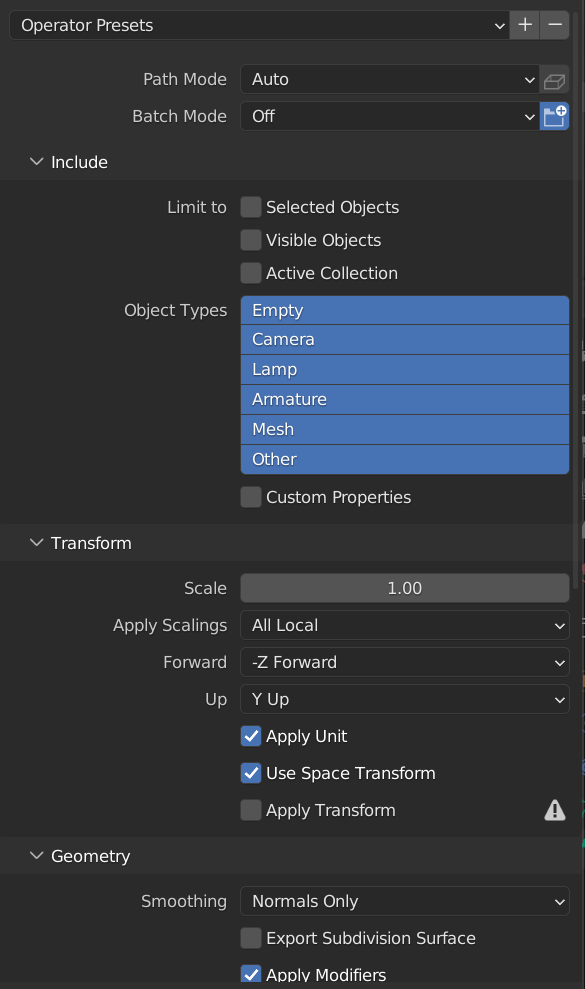
\includegraphics[width=0.47\textwidth]{resources/chapter-4/export-fbx-options-1.png}}
    \hfill
    \subfloat[Opsi ekspor berkas FBX lanjutan]{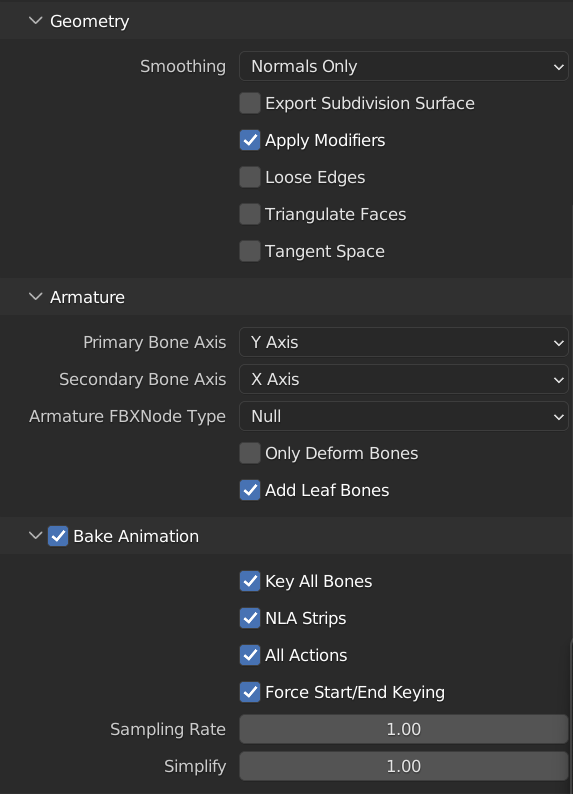
\includegraphics[width=0.47\textwidth]{resources/chapter-4/export-fbx-options-2.png}}
    \caption{Opsi ekspor berkas FBX}
    \label{fig:export-fbx}
\end{figure}

\subsubsection{Pengimporan Berkas FBX dan Konfigurasi Kendaraan Roda 4 dalam Editor CARLAUE4}

% note: add carlaue4 editor ui?

Setelah aset model 3D selesai dibuat dan diekspor ke dalam format FBX, berkas
FBX tersebut diimpor ke dalam editor CARLAUE4. Sebelum berkas FBX kendaraan
diimpor, sebuah \textit{folder} baru dibuat di dalam direktori
\verb|/Content/Carla/Static/Vehicles/4Wheeled/| (selanjutnya akan disebut
sebagai \textit{folder} \verb|Static|) di \textit{Content Browser} kemudian
berkas FBX dapat diimpor ke dalam \textit{folder} tersebut dengan klik kanan
pada \textit{Content Browser}. Gambar \ref{fig:fbx-import-options-4wheeled}
menunjukkan opsi yang digunakan untuk mengimpor berkas FBX kendaraan roda 4.
Berikut adalah beberapa opsi yang perlu diperhatikan dan diatur:

\begin{enumerate}
    \item Opsi \verb|Import Content Type| diatur ke \texttt{Geometry and Skinning Weights}.
    \item Opsi \verb|Normal Import Method| diatur ke \verb|Import Normals|.
    \item Opsi \verb|Use T0 as Ref Pose| dicentang.
\end{enumerate}

\begin{figure}[!ht]
    \centering
    \subfloat[Opsi impor berkas FBX]{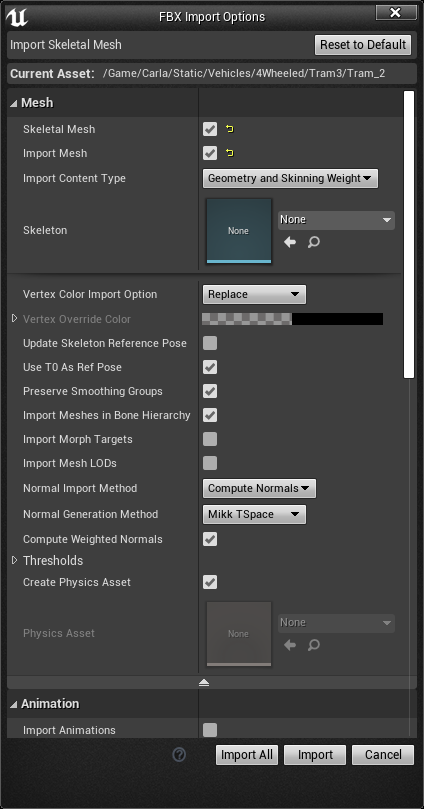
\includegraphics[width=0.47\textwidth]{resources/chapter-4/fbx-import-options-4wheeled-1.png}}
    \hfill
    \subfloat[Opsi impor berkas FBX lanjutan]{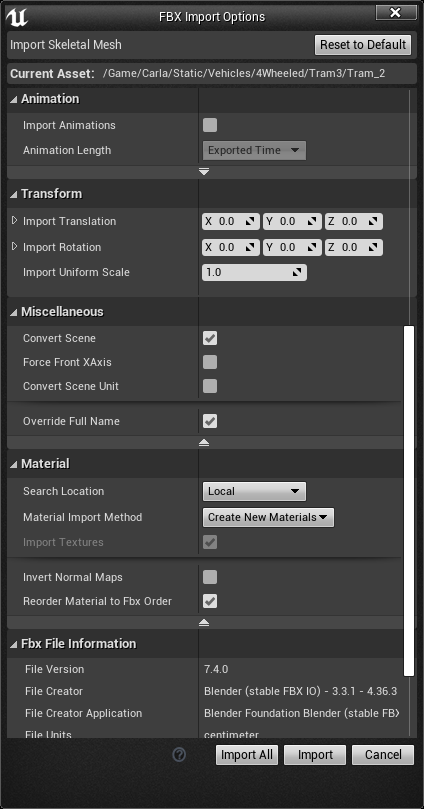
\includegraphics[width=0.47\textwidth]{resources/chapter-4/fbx-import-options-4wheeled-2.png}}
    \caption{Opsi impor berkas FBX kendaraan roda 4}
    \label{fig:fbx-import-options-4wheeled}
\end{figure}

Pengimporan berkas FBX tersebut menghasilkan aset-aset sebagai berikut:

\begin{enumerate}
    \item Aset \textit{skeletal mesh} \verb|<nama_kendaraan>|
    \item Aset \textit{skeleton} \verb|<nama_kendaraan>_Skeleton|
    \item Aset \textit{physics} \verb|<nama_kendaraan>_PhysicsAsset|
    \item Aset-aset material dan tekstur yang ada dalam berkas FBX jika opsi
    \verb|Material Import Method| diatur ke \verb|Create New Materials|.
\end{enumerate}

Aset \textit{physics} diedit agar sesuai dengan bentuk aset \textit{mesh}.
Bentuk \textit{body} badan kendaraan atau \textit{vehicle base} disesuaikan
dengan cara mengubah \verb|Primitive Type| menjadi \verb|Multi Convex Hull|
pada panel \verb|Tools|. Badan dari masing-masing roda kendaraan disesuaikan
bentuk \verb|Primitive Type|-nya menjadi \verb|Sphere|. Dilakukan pengaturan
opsi-opsi pada panel \verb|Details| untuk masing-masing roda, yaitu opsi
\verb|Linear Damping| diatur menjadi \verb|0| dan opsi \verb|Physics Type|
diatur menjadi \verb|Kinematic|. Opsi \verb|Simulation Generates Hit Events|
pada panel \verb|Details| dicentang untuk badan dan roda-roda kendaraan agar
\textit{collider} kendaraan dapat menghasilkan \textit{hit event}. Gambar
\ref{fig:physics-asset-4wheeled} menunjukkan aset \textit{physics} kendaraan
roda 4 sebelum dan setelah diedit.

\begin{figure}[!ht]
    \centering
    \subfloat[Aset \textit{physics} trem sebelum pengeditan]{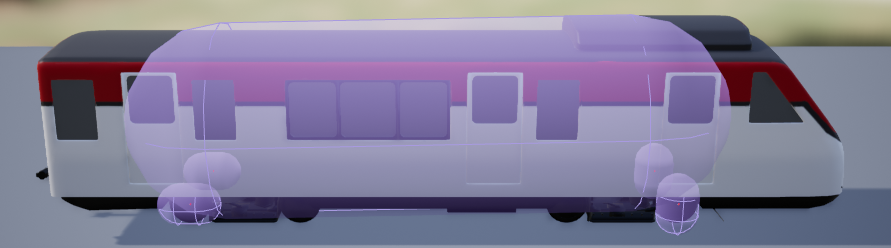
\includegraphics[width=0.6\textwidth]{resources/chapter-4/tram-physics-asset-before.png}}
    \hfill
    \subfloat[Aset \textit{physics} trem setelah pengeditan]{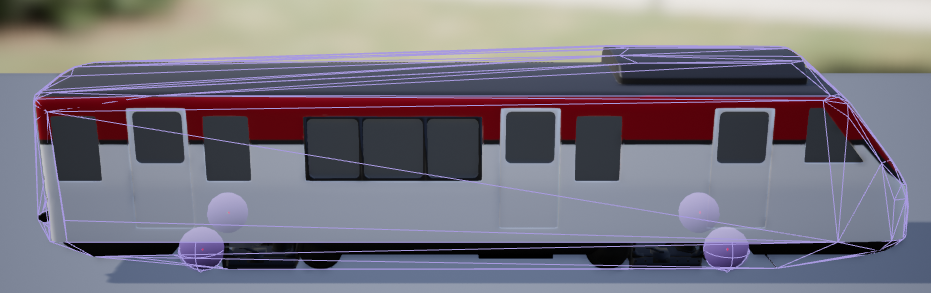
\includegraphics[width=0.6\textwidth]{resources/chapter-4/tram-physics-asset-after.png}}
    \caption{Aset \textit{physics} trem}
    \label{fig:physics-asset-4wheeled}
\end{figure}

Selain pengeditan aset \textit{physics}, dilakukan pembuatan aset \textit{static
mesh} dan berbagai aset \textit{blueprint} agar aset kendaraan dapat
mengintegrasikan sebagai kendaraan. Aset \textit{static mesh} dibuat dengan cara
menekan tombol \verb|Make Static Mesh| pada panel \verb|Toolbar| pada aset
\textit{skeletal mesh}. Aset tersebut dibuat untuk melengkapi \textit{static
mesh} yang tidak dibuat dalam Blender. Aset tersimpan pada direktori
\verb|/Content/Meshes/| dengan nama \verb|<nama_kendaraan>|.

Aset \textit{animation blueprint} dibuat untuk mengatur animasi kendaraan.
Karena semua animasi kendaraan roda 4 sama, aset \textit{animation blueprint}
dapat dibuat dengan menyalin isi aset \textit{animation blueprint} dari salah
satu kendaraan roda 4 yang sudah ada kemudian aset di-\textit{compile} dan
disimpan dengan nama \verb|AnimBP_<nama_kendaraan>|. Gambar
\ref{fig:blueprint-animation-4wheeled} menunjukkan aset \textit{animation
blueprint} trem.

\begin{figure}[!h]
    \centering
    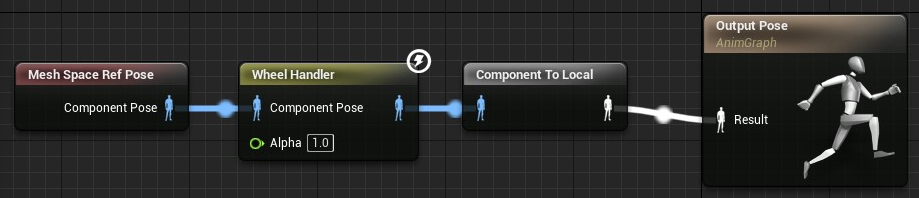
\includegraphics[width=1\textwidth]{resources/chapter-4/tram-animation-blueprint.png}
    \caption{Aset \textit{animation blueprint} trem}
    \label{fig:blueprint-animation-4wheeled}
\end{figure}

% note: blueprint animation can be explained more in detail

Aset-aset di dalam \textit{folder} \verb|Static| selesai dibuat. Gambar
\ref{fig:tram-assets-in-static-folder} menunjukkan aset-aset trem dalam
\textit{folder} \verb|Static|.

\begin{figure}[!h]
    \centering
    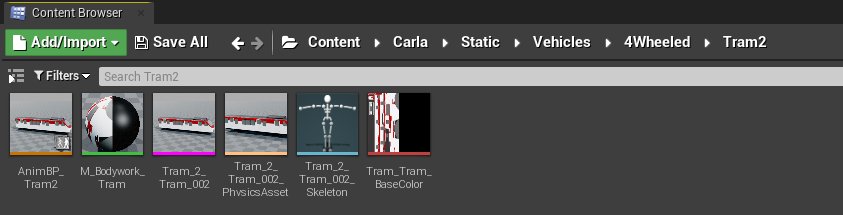
\includegraphics[width=1\textwidth]{resources/chapter-4/tram-assets-in-static-folder.png}
    \caption{Aset-aset trem dalam \textit{folder} \texttt{Static}}
    \label{fig:tram-assets-in-static-folder}
\end{figure}

Selanjutnya, dilakukan pembuatan 5 aset dalam direktori
\verb|/Content/Carla/Blueprints/Vehicle/<nama_kendaraan>/| (selanjutnya akan
disebut sebagai \textit{folder} \verb|Blueprints|). Lima aset tersebut adalah
aset 4 \textit{blueprint} roda dan 1 aset \textit{blueprint} kendaraan. Empat
aset \textit{blueprint} roda dibuat dengan klik kanan pada \textit{Content
Browser} dan memilih opsi \verb|Blueprint Class| kemudian memilih
\verb|VehicleWheel| untuk opsi \verb|Parent Class|. Masing-masing aset diberi
nama \verb|BP_<nama_kendaraan>_<posisi_roda>| dengan posisi roda: \verb|FLW|
(\textit{front left wheel}), \verb|FRW| (\textit{front right wheel}), \verb|RLW|
(\textit{rear left wheel}), atau \verb|RRW| (\textit{rear right wheel}).
Aset-aset \textit{blueprint} roda dibuka dan diatur nilai-nilainya pada panel
\verb|Class Defaults| dengan konfigurasi sebagai berikut:

\begin{enumerate}
    \item Opsi \verb|Collision Mesh| diatur menjadi \verb|Wheel_Shape|
    \item Opsi \verb|Shape Radius| diatur sesuai dengan radius roda
    \item Opsi \verb|Shape Width| diatur sesuai dengan ketebalan roda
    \item Opsi \verb|Mass| diatur sesuai dengan massa roda dalam kilogram
    \item Opsi \verb|Steer Angle| diatur menjadi \verb|70| (derajat) untuk roda
    depan dan \verb|0| (derajat) untuk roda belakang
    \item Opsi \verb|Affected by Handbrake| tidak dicentang untuk roda depan dan
    dicentang untuk roda belakang
    \item Opsi \verb|Tire Config| diatur menjadi \verb|CommonTireConfig|
\end{enumerate}

Aset-aset \textit{blueprint} roda selesai dibuat. Gambar
\ref{fig:tram-wheel-blueprints} menunjukkan isi dari 2 \textit{blueprint} roda
trem, yaitu roda kiri depan dan roda kiri belakang.

\begin{figure}[!ht]
    \centering
    \subfloat[Aset \textit{blueprint} roda kiri depan trem]{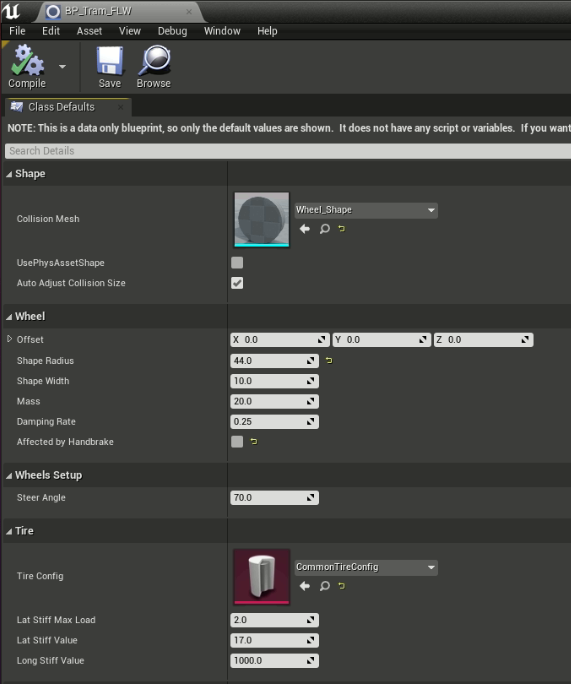
\includegraphics[width=0.47\textwidth]{resources/chapter-4/tram-wheel-bp-flw.png}}
    \hfill
    \subfloat[Aset \textit{blueprint} roda kiri belakang trem]{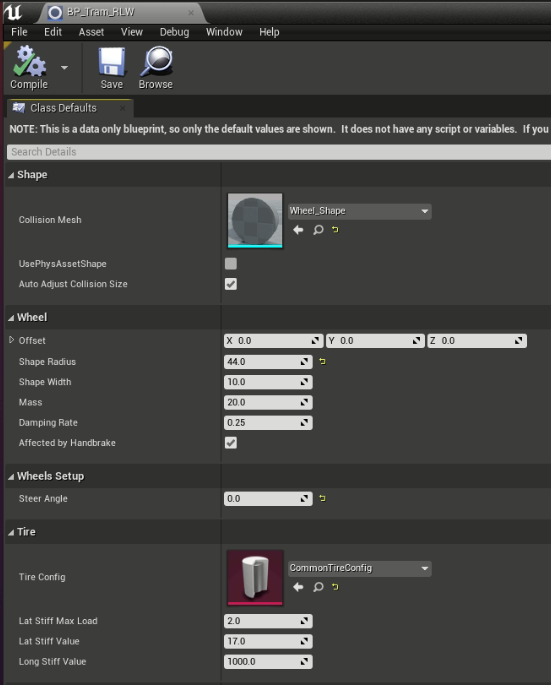
\includegraphics[width=0.47\textwidth]{resources/chapter-4/tram-wheel-bp-rlw.png}}
    \caption{Aset \textit{blueprint} roda trem}
    \label{fig:tram-wheel-blueprints}
\end{figure}

Setelah semua opsi diatur, aset-aset \textit{blueprint} roda di-\textit{compile}
dan disimpan. Selanjutnya, aset \textit{blueprint} kendaraan dibuat dengan klik
kanan pada \textit{Content Browser} dan memilih opsi \verb|Blueprint Class|
kemudian memilih \verb|BaseVehiclePawn| untuk opsi \verb|Parent Class|. Aset
diberi nama \verb|BP_<nama_kendaraan>|. Aset \textit{blueprint} kendaraan roda 4
diatur dengan konfigurasi sebagai berikut:

\begin{enumerate}
    \item Pada komponen \verb|Mesh (VehicleMesh) Inherited|, opsi \verb|Skeletal Mesh|
    diatur menjadi aset \textit{skeletal mesh} \verb|<nama_kendaraan>|
    \item Pada komponen \verb|Mesh (VehicleMesh) Inherited|, opsi \verb|Anim Class|
    diatur menjadi aset \textit{animation blueprint}
    \verb|AnimBP_<nama_kendaraan>|
    \item Pada komponen \verb|Custom Collision (Inherited)|, opsi \verb|Static Mesh|
    diatur menjadi aset \textit{static mesh} \verb|<nama_kendaraan>|
    \item Pada komponen \verb|VehicleMovement (MovementComp) (Inherited)|, 4
    opsi \verb|Wheel Class| diatur menjadi aset-aset \textit{blueprint} roda
    sesuai dengan posisi roda. Gambar \ref{fig:tram-blueprint-wheels}
    menunjukkan konfigurasi roda.
\end{enumerate}

\begin{figure}[!h]
    \centering
    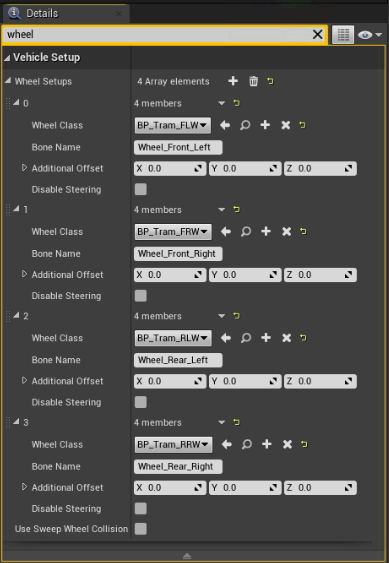
\includegraphics[width=0.47\textwidth]{resources/chapter-4/tram-blueprint-wheels.png}
    \caption{Konfigurasi roda pada \textit{blueprint} kendaraan trem}
    \label{fig:tram-blueprint-wheels}
\end{figure}

Aset-aset di dalam \textit{folder} \verb|Blueprints| selesai dibuat. Gambar
\ref{fig:tram-assets-in-blueprints-folder} menunjukkan aset-aset trem dalam
\textit{folder} \verb|Blueprints|.

\begin{figure}[!h]
    \centering
    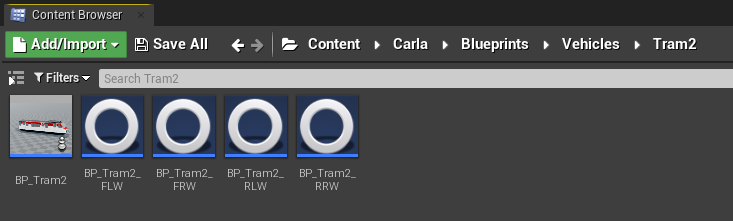
\includegraphics[width=1\textwidth]{resources/chapter-4/tram-assets-in-blueprints-folder.png}
    \caption{Aset-aset trem dalam \textit{folder} \texttt{Blueprints}}
    \label{fig:tram-assets-in-blueprints-folder}
\end{figure}

Setelah semua aset \textit{blueprint} dibuat, di-\textit{compile}, dan disimpan,
\textit{blueprint} kendaraan dimasukkan ke dalam berkas \verb|VehicleFactory|
yang terletak di dalam \verb|/Content/Carla/Blueprints/Vehicle/| agar dapat
dimunculkan atau di-\textit{spawn} di dalam simulasi. \textit{Blueprint}
kendaraan sebagai sebuah elemen baru dalam \textit{array} kendaraan.

Gambar \ref{fig:tram-carla} menunjukkan hasil implementasi trem. Gambar
\ref{fig:angkot-carla} menunjukkan hasil implementasi trem  angkot.

\begin{figure}[!h]
    \centering
    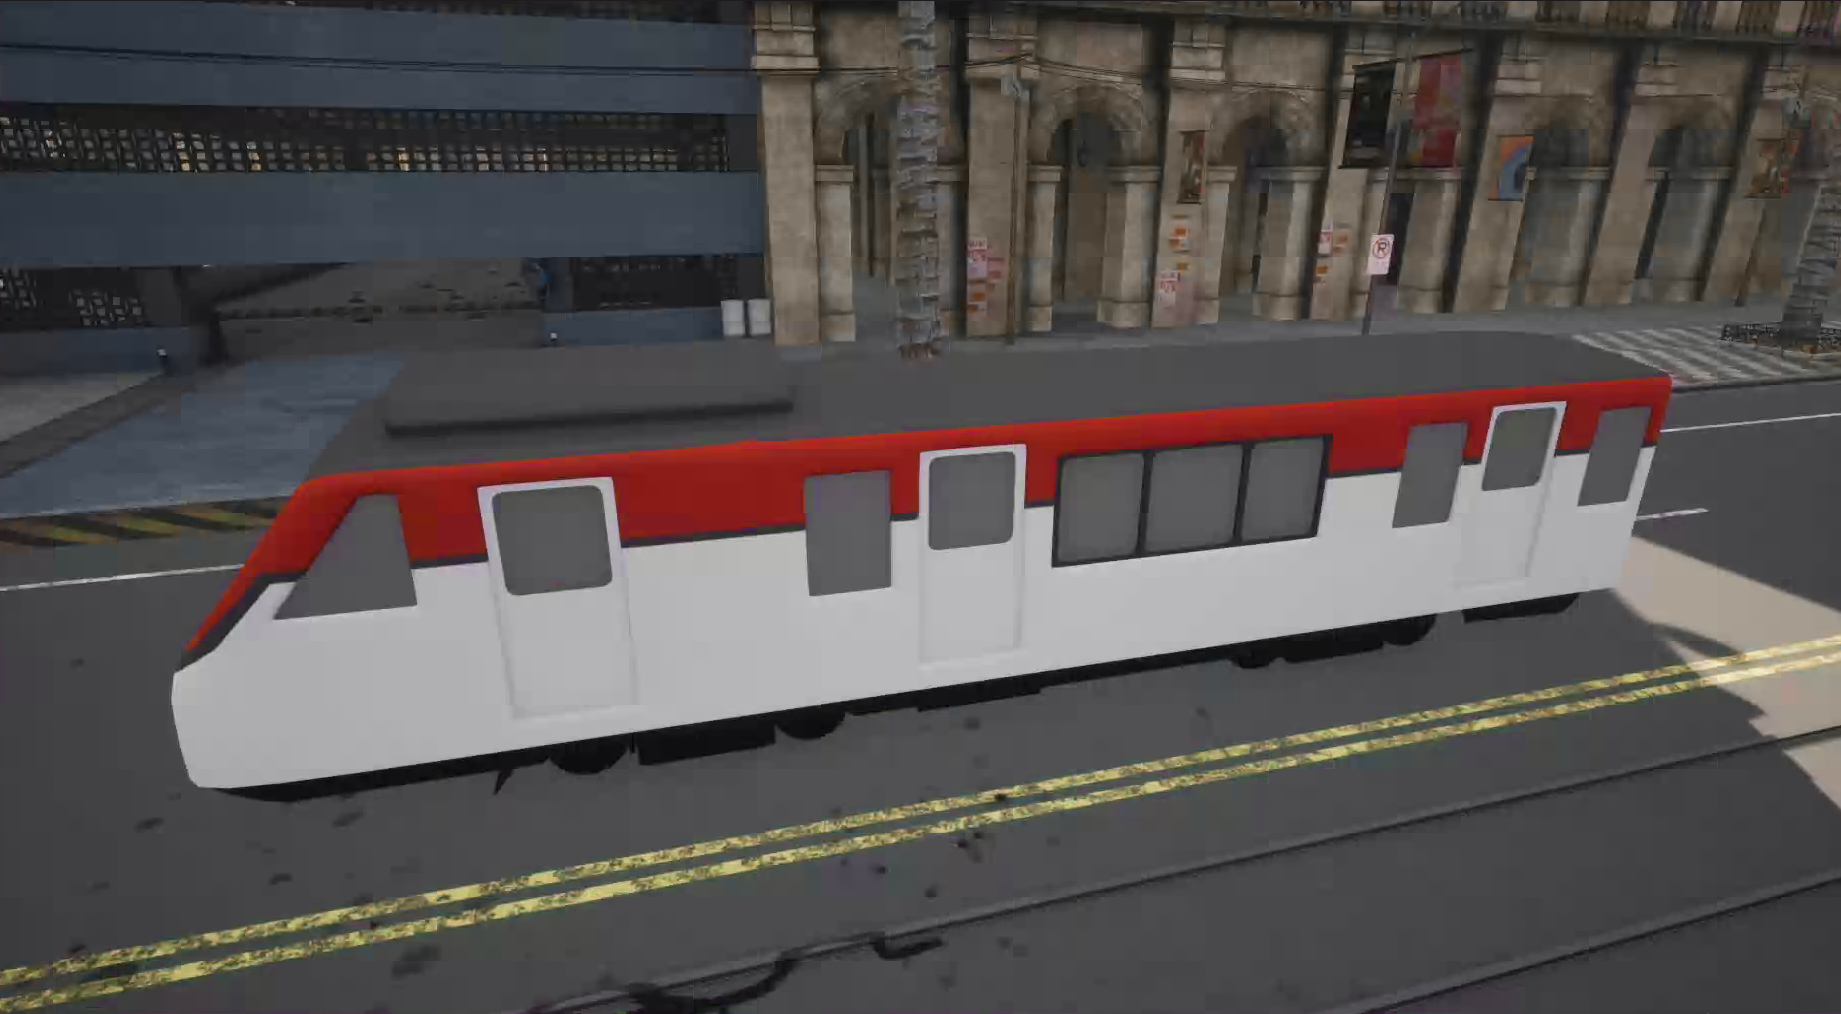
\includegraphics[width=0.6\textwidth]{resources/chapter-4/tram-carla.png}
    \caption{Implementasi trem dalam lingkungan simulasi}
    \label{fig:tram-carla}
\end{figure}

\begin{figure}[!h]
    \centering
    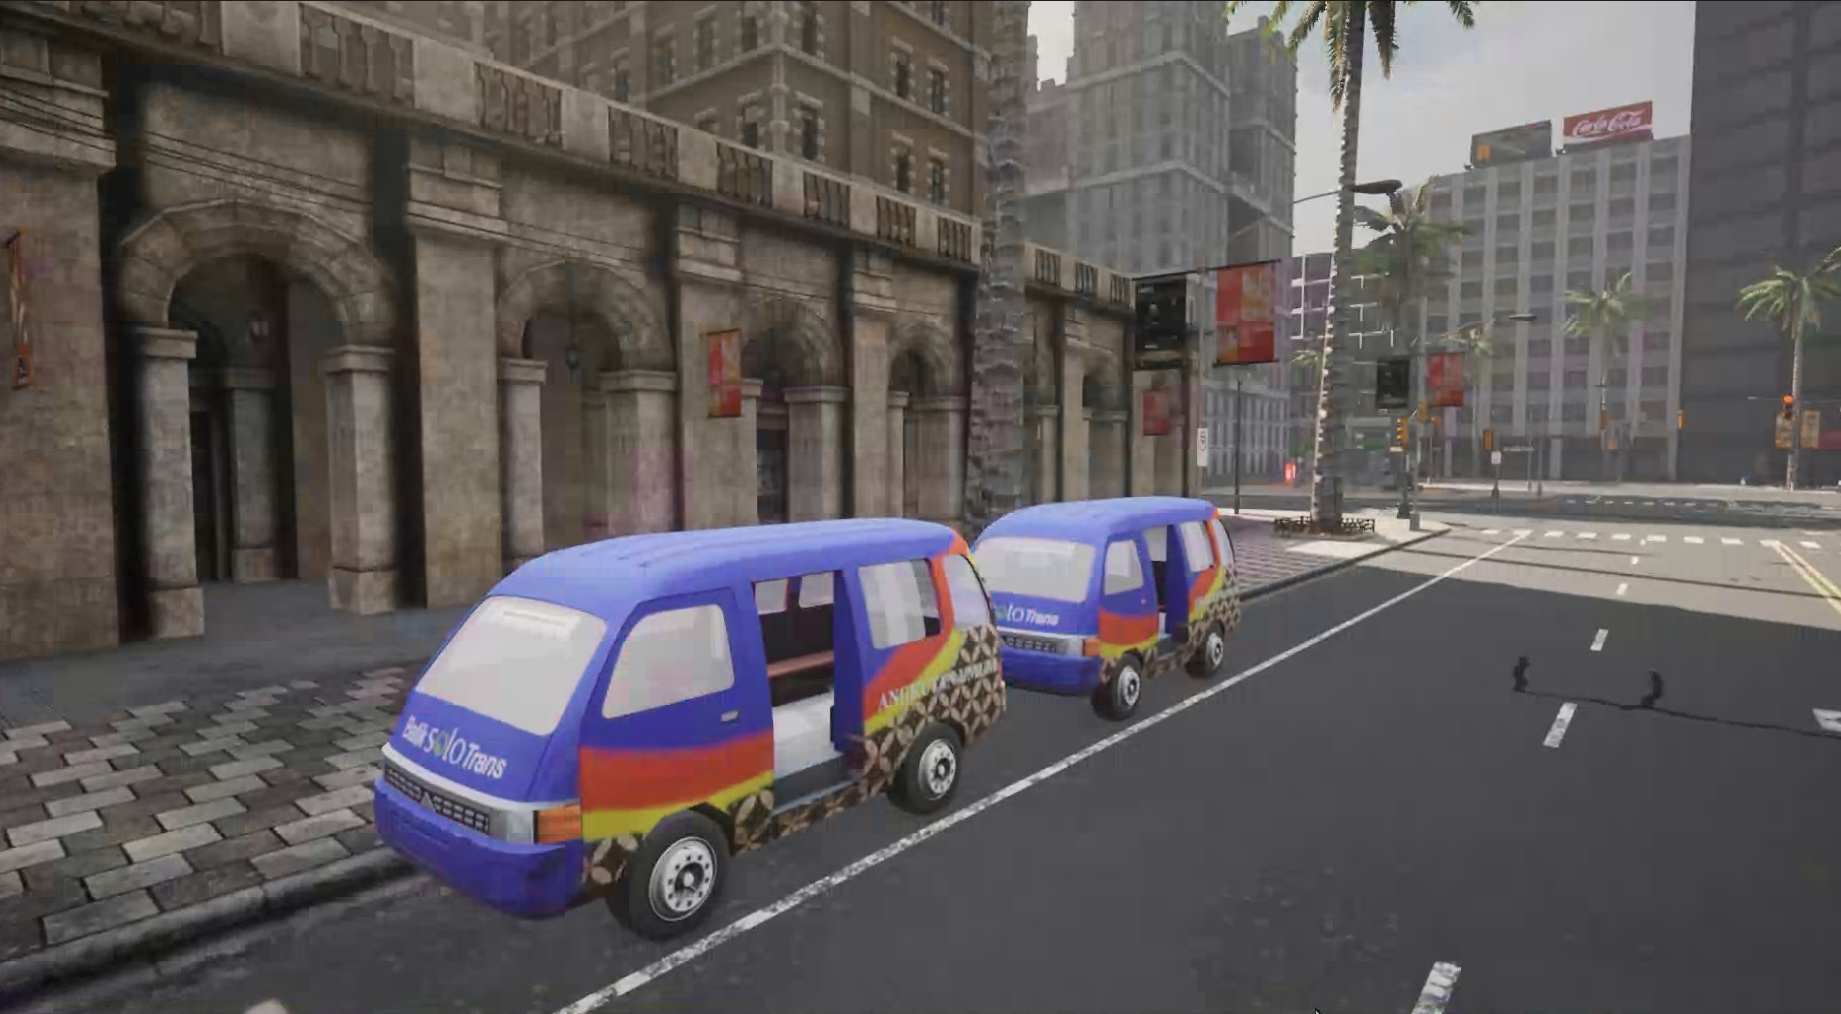
\includegraphics[width=0.6\textwidth]{resources/chapter-4/angkot.png}
    \caption{Implementasi angkot dalam lingkungan simulasi}
    \label{fig:angkot-carla}
\end{figure}

\subsection{Implementasi Sepeda Onthel, Sepeda Motor, dan Becak}

Implementasi sepeda onthel, sepeda motor, dan becak sebagai kendaraan roda 2
terbagi menjadi dua bagian, yaitu: pembuatan aset model 3D untuk ekspor berkas
FBX, dan pengimporan berkas FBX dan konfigurasi kendaraan roda 2 dalam editor
CARLAUE4.

\subsubsection{Pembuatan Aset Model 3D untuk Ekspor berkas FBX}

Pembuatan aset model 3D untuk kendaraan roda 2 dilakukan dengan cara yang serupa
dengan pembuatan aset model 3D untuk kendaraan roda 4. Perbedaannya terletak
pada \textit{armature} yang digunakan dan proses \textit{skinning}. Gambar
\ref{fig:bike-skeleton} menunjukkan \textit{armature} kendaraan roda 2/sepeda.
Sebelum proses \textit{skinning}, setiap \textit{bone} diatur posisinya
masing-masing agar sesuai. Masing-masing \textit{vertices groups} dibuat untuk
setiap \textit{bone} yang perlu dihubungkan dengan \textit{mesh}, yaitu:

\begin{enumerate}
    \item \verb|BikeBodyGeo| dengan seluruh \textit{mesh} kendaraan selain roda
    \item \verb|HandlerGeo| dengan \textit{mesh} roda depan dan pegangan
    kendaraan
    \item \verb|PedalsGeo| dengan \textit{mesh} \textit{pedalier}
    \item \verb|FrontWheelGeo| dengan \textit{mesh} roda depan
    \item \verb|RearWheelGeo| dengan \textit{mesh} roda belakang
\end{enumerate}

\begin{figure}[!h]
    \centering
    \subfloat[\textit{Armature}]{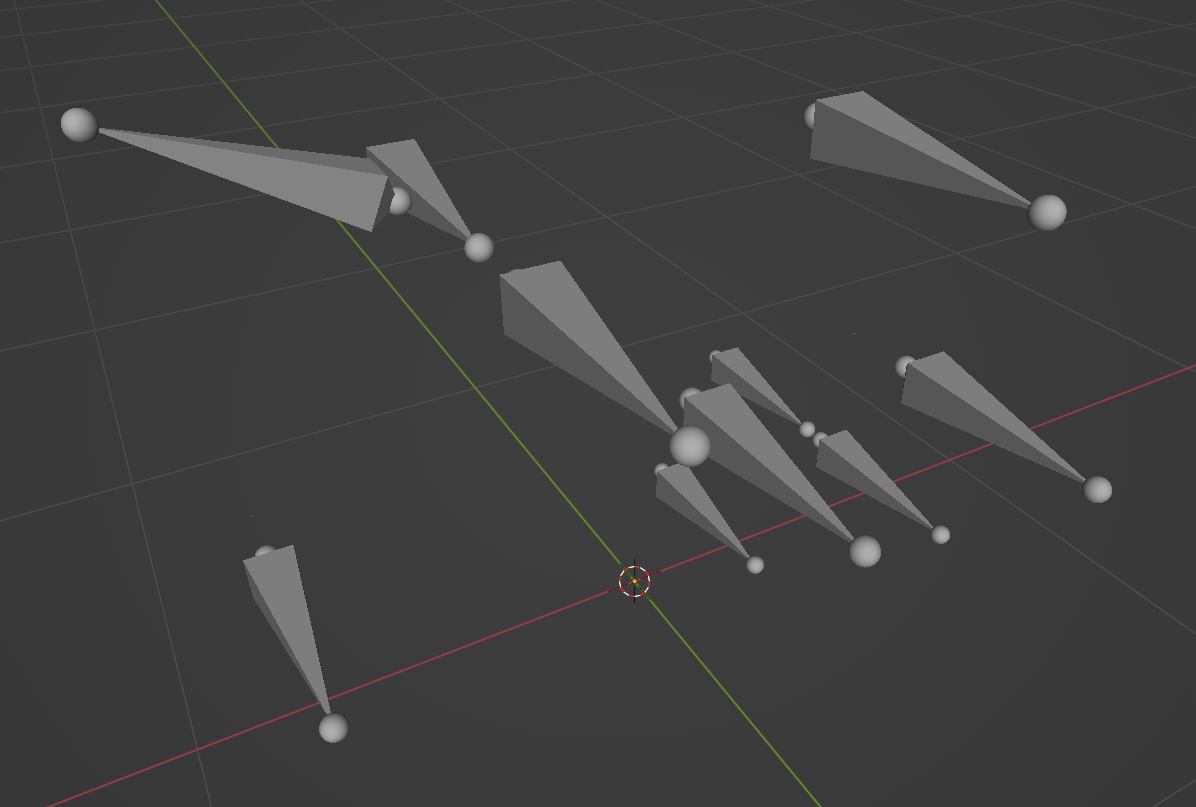
\includegraphics[width=0.5\textwidth]{resources/chapter-4/bike-skeleton.png}}
    \hfill
    \subfloat[Hierarki \textit{bike skeleton}]{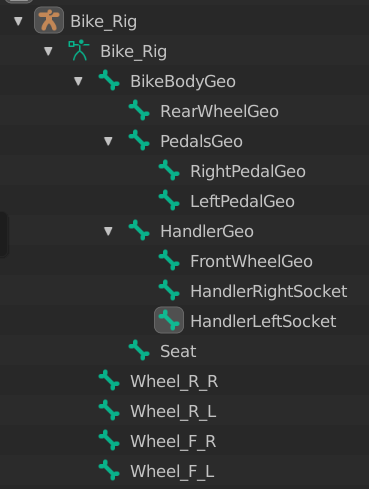
\includegraphics[width=0.35\textwidth]{resources/chapter-4/bike-skeleton-hierarchy.png}}
    \caption{\textit{Vehicle skeleton} kendaraan roda 4}
    \label{fig:bike-skeleton}
\end{figure}

Gambar \ref{fig:onthel-model-with-armature} menunjukkan hasil \textit{skinning}.
Setelah proses \textit{skinning} aset diekspor dengan opsi yang sama
dengan ekspor berkas FBX untuk kendaraan roda 4. Gambar \ref{fig:export-fbx}
menunjukkan opsi yang digunakan.

\begin{figure}[!h]
    \centering
    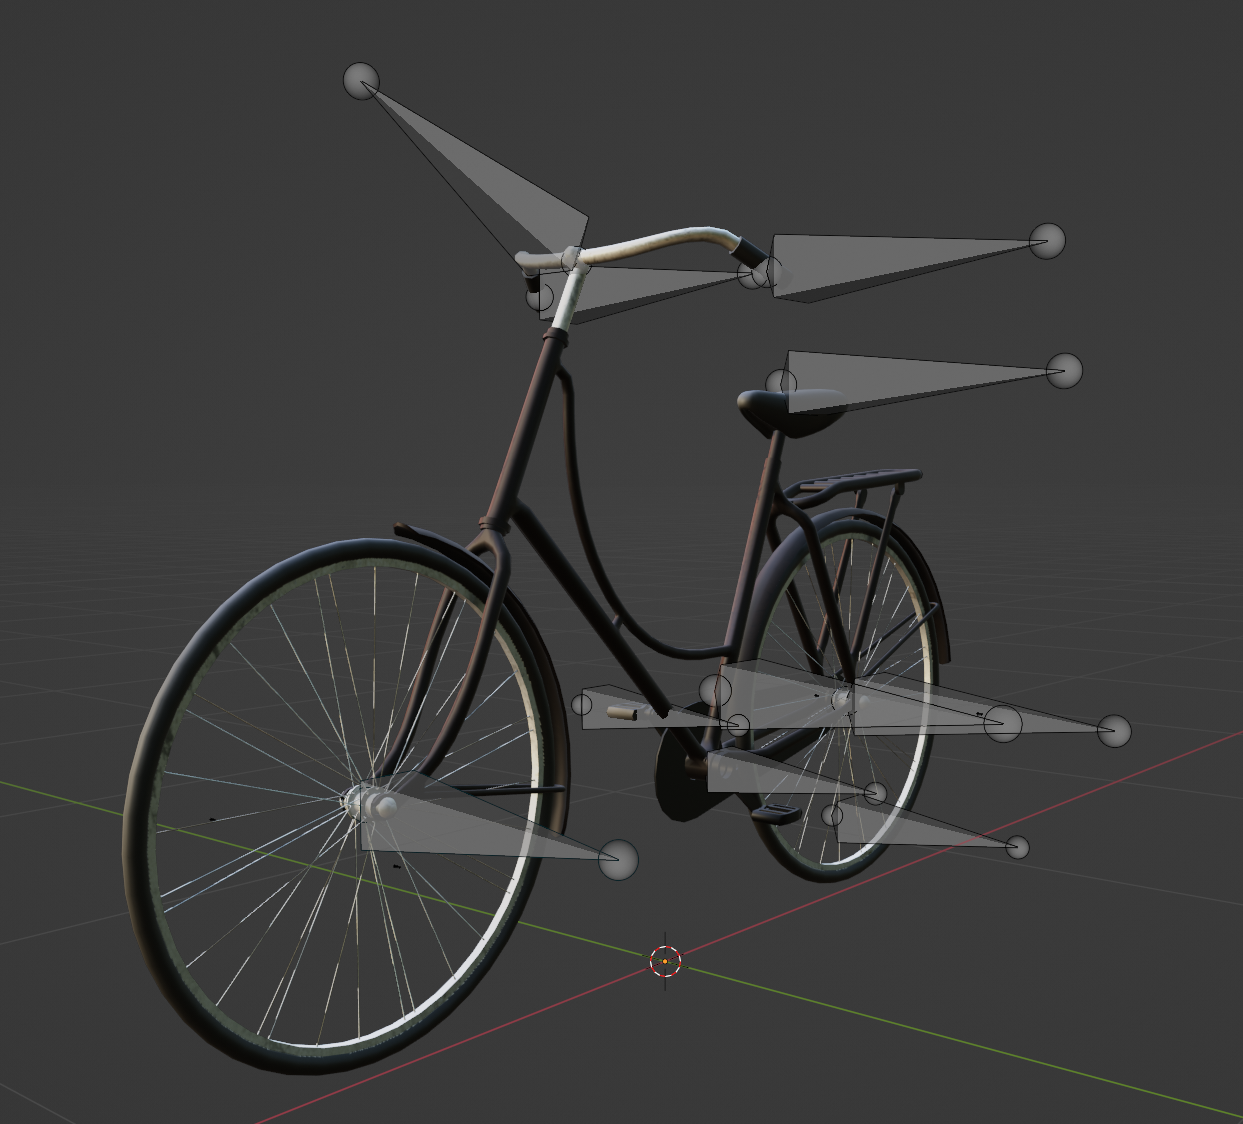
\includegraphics[width=0.5\textwidth]{resources/chapter-4/sepeda-onthel-model-2.png}
    \caption{Aset model 3D sepeda onthel dengan \textit{armature}}
    \label{fig:onthel-model-with-armature}
\end{figure}

\subsubsection{Pengimporan Berkas FBX dan Konfigurasi Kendaraan Roda 2 dalam Editor CARLAUE4}

Berkas FBX kendaraan roda 2 diimpor ke dalam \textit{folder} baru untuk
masing-masing kendaraan di dalam direktori
\verb|/Content/Carla/Static/Vehicles/2Wheeled/| (selanjutnya akan disebut
sebagai \textit{folder} \verb|Static|). Opsi yang digunakan untuk impor berkas
FBX adalah:

\begin{enumerate}
    \item Opsi \verb|Import Content Type| diatur ke \texttt{Geometry and Skinning Weights}
    \item Opsi \verb|Skeleton| diatur ke aset \textit{skeleton} \verb|4WheeledBike|
    \item Opsi \verb|Normal Import Method| diatur ke \verb|Import Normals|
    \item Opsi \verb|Use T0 as Ref Pose| dicentang
\end{enumerate}

Setelah berkas FBX diimpor, muncul aset \textit{skeletal mesh}, aset
\textit{physics}, aset material, dan aset tekstur. Aset \textit{skeleton} tidak
dihasilkan oleh impor sebab telah diatur pada opsi \verb|Skeleton| saat impor.
Gambar \ref{fig:onthel-assets-in-static-folder} menunjukkan aset yang dihasilkan
oleh impor berkas FBX.

\begin{figure}[!h]
    \centering
    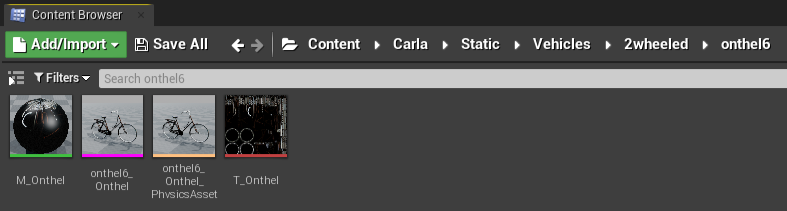
\includegraphics[width=1\textwidth]{resources/chapter-4/onthel-assets-in-static-folder.png}
    \caption{Aset-aset sepeda onthel dalam \textit{folder} \texttt{Static}}
    \label{fig:onthel-assets-in-static-folder}
\end{figure}

Aset \textit{physics} juga perlu diatur agar sesuai dengan bentuk kendaraan.
Bentuk badan kendaraan roda 2 diatur agar sesuai dengan mengatur opsi
\verb|Primitive Type| menjadi \verb|Multi Convex Hull| pada panel \verb|Tools|.
Selain itu opsi \verb|Simulate Generates Hit Events| dicentang pada panel
\verb|Details|. Kedua roda kendaraan diatur bentuknya juga dengan mengatur opsi
\verb|Primitive Type| menjadi \verb|Sphere|. Opsi \verb|Simulate Generates Hit Events|
juga dicentang. Opsi \verb|Physics Type| diatur menjadi \verb|Kinematic| untuk
kedua roda. Gambar \ref{fig:physics-asset-2wheeled} menunjukkan hasil
konfigurasi aset \textit{physics} kendaraan roda 2.

\begin{figure}[!h]
    \centering
    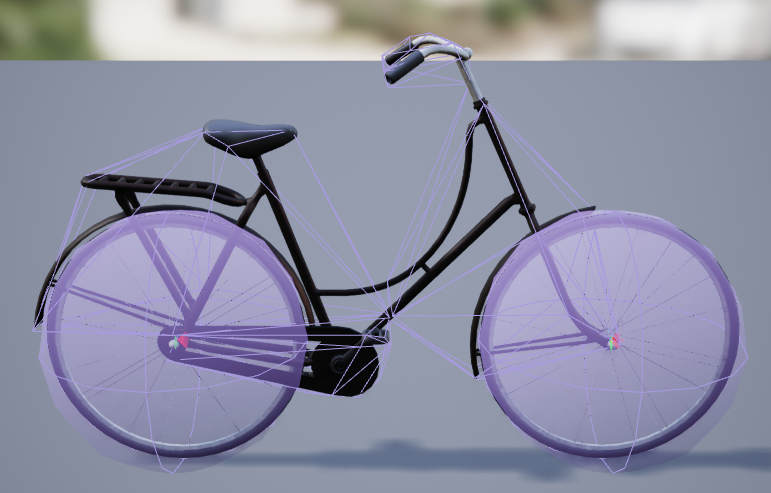
\includegraphics[width=0.5\textwidth]{resources/chapter-4/onthel-physics-asset.png}
    \caption{Aset \textit{physics} sepeda onthel}
    \label{fig:physics-asset-2wheeled}
\end{figure}

Dibuat aset \textit{static mesh} untuk melengkapi kendaraan roda 2. Aset ini
terletak di dalam \textit{folder} \verb|/Content/Meshes/| dengan nama
\verb|<nama_kendaraan>|.

Aset \textit{animation blueprint} tidak perlu dibuat karena menggunakan aset
\textit{animation blueprint} kendaraan roda 2 yang sudah disediakan oleh CARLA.
Selanjutnya, dibuat aset-aset \textit{blueprint} dalam direktori
\verb|/Content/Carla/Blueprints/Vehicle/2Wheeled/<nama_kendaraan>| (selanjutnya
akan disebut sebagai \textit{folder} \verb|Blueprints|). Dibuat 2 aset
\textit{blueprint} untuk roda depan dan roda belakang. Cara pembuatan dan
konfigurasi aset roda sama dengan cara pembuatan dan konfigurasi aset
\textit{blueprint} roda pada kendaraan roda 4. Gambar
\ref{fig:onthel-wheel-blueprints} menunjukkan kedua aset \textit{blueprint} roda
dengan nama \verb|<nama_kendaraan>_FrontWheel>| dan
\verb|<nama_kendaraan>_RearWheel>|.

\begin{figure}[!ht]
    \centering
    \subfloat[Aset \textit{blueprint} roda depan onthel]{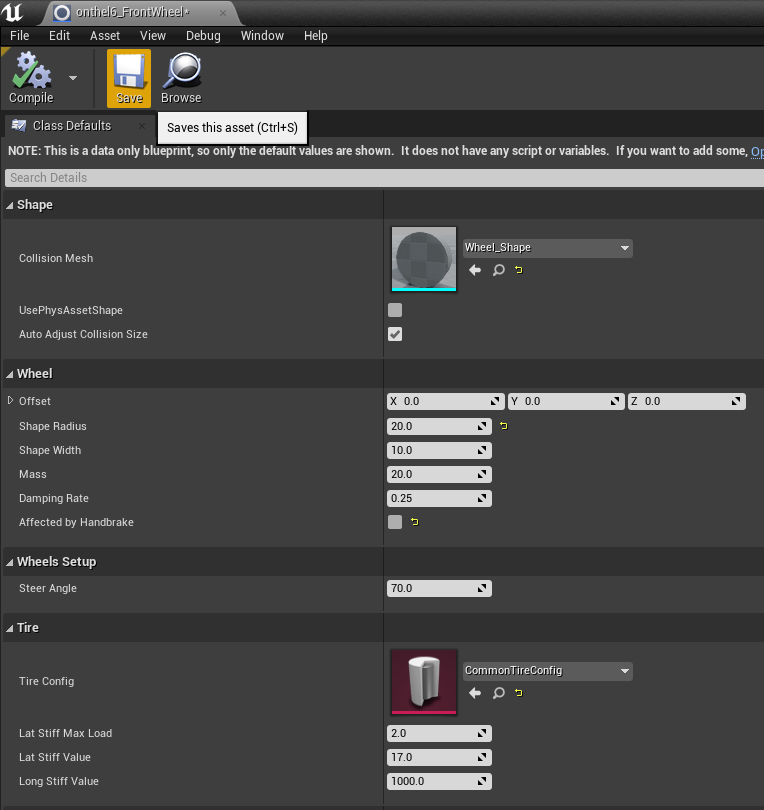
\includegraphics[width=0.47\textwidth]{resources/chapter-4/onthel-wheel-bp-fw.png}}
    \hfill
    \subfloat[Aset \textit{blueprint} roda belakang onthel]{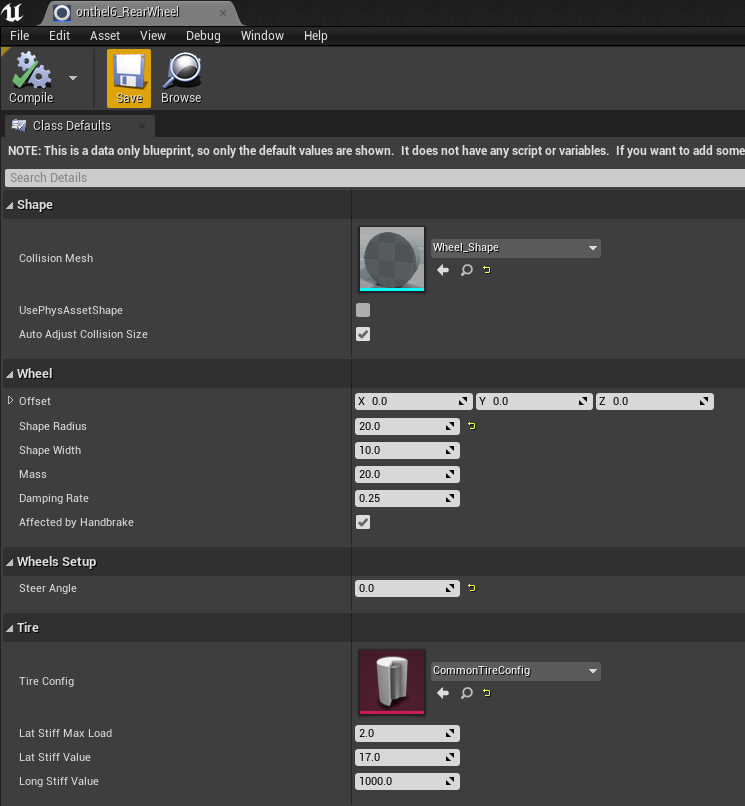
\includegraphics[width=0.47\textwidth]{resources/chapter-4/onthel-wheel-bp-rw.png}}
    \caption{Aset \textit{blueprint} roda onthel}
    \label{fig:onthel-wheel-blueprints}
\end{figure}

Dibuat aset \textit{blueprint} untuk kendaraan roda 2 dengan nama
\verb|<nama_kendaraan>| dalam direktori yang sama. Aset \textit{blueprint}
tersebut dibuat dengan opsi \verb|Parent Class| diatur menjadi
\verb|BP_Base2wheeledNew|. Aset \textit{blueprint} kendaraan roda 2
diatur dengan konfigurasi sebagai berikut:

\begin{enumerate}
    \item Pada komponen \verb|Mesh (VehicleMesh) Inherited|, opsi \verb|Skeletal Mesh|
    diatur menjadi aset \textit{skeletal mesh} \verb|<nama_kendaraan>|
    \item Pada komponen \verb|Mesh (VehicleMesh) Inherited|, opsi \verb|Anim Class|
    diatur menjadi aset \textit{animation blueprint} \verb|4WheeledBike_Anim|
    \item Pada komponen \verb|Custom Collision (Inherited)|, opsi \verb|Static Mesh|
    diatur menjadi aset \textit{static mesh} \verb|<nama_kendaraan>|
    \item Pada komponen \verb|VehicleMovement (MovementComp) (Inherited)|, 2
    opsi \verb|Wheel Class| pertama diatur menjadi aset \textit{blueprint} roda
    depan dan 2 opsi terakhir diubah menjadi aset \textit{blueprint} roda
    belakang.
    \item Pada komponen \verb|VehicleMovement (MovementComp) (Inherited)|, 2
    opsi \verb|Bone Name| diubah menjadi \verb|FrontWheelGeo| dan 2 opsi
    \verb|Bone Name| diubah menjadi \verb|RearWheelGeo|. Gambar
    \ref{fig:onthel-blueprint-wheels} menunjukkan konfigurasi roda.
    \item Pada komponen \verb|SkeletalMesh (Inherited)|, opsi \verb|Rotation|
    diubah hingga \textit{mesh} pengemudi duduk tegak.
\end{enumerate}

Aset-aset di dalam \textit{folder} \verb|Blueprints| selesai dibuat. Gambar
\ref{fig:onthel-assets-in-blueprints-folder} menunjukkan aset-aset onthel dalam
\textit{folder} \verb|Blueprints|.

\begin{figure}[!h]
    \centering
    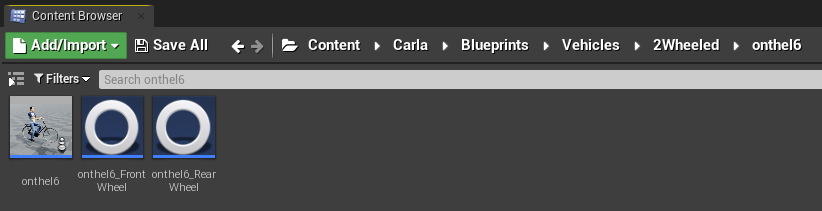
\includegraphics[width=1\textwidth]{resources/chapter-4/onthel-assets-in-blueprints-folder.png}
    \caption{Aset-aset onthel dalam \textit{folder} \texttt{Blueprints}}
    \label{fig:onthel-assets-in-blueprints-folder}
\end{figure}

Aset \textit{blueprint} kendaraan roda 2 dimasukkan kedalam berkas
\verb|VehicleFactory| agar kendaraan roda 2 dapat di-\textit{spawn} dalam
simulasi. Gambar \ref{fig:onthel-carla} menunjukkan hasil implementasi kendaraan
roda 2 dalam simulasi.

\begin{figure}[!h]
    \centering
    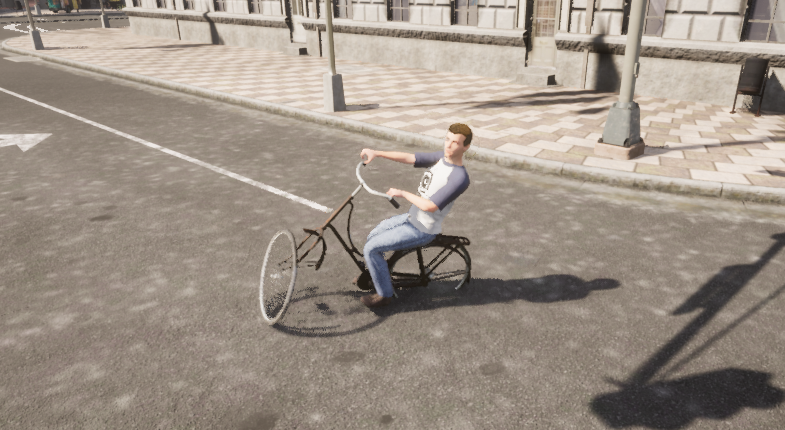
\includegraphics[width=0.6\textwidth]{resources/chapter-4/onthel-carla.png}
    \caption{Implementasi onthel dalam lingkungan simulasi}
    \label{fig:onthel-carla}
\end{figure}

\subsection{Implementasi Lingkungan}

Penambahan aset model 3D ke dalam lingkungan simulasi dilakukan dengan membuat
\textit{folder} baru untuk masing-masing objek/\textit{mesh}/\textit{static
mesh} dalam \textit{folder} \verb|Static| kemudian mengimpor aset model 3D ke
dalam masing-masing \textit{folder} tersebut. Objek statis ditambahkan dengan
cara menarik berkas objek dari \textit{Content Browser} ke dalam
\textit{Viewport}. Setelah itu, dapat dilakukan penyesuaian skala, posisi, dan
rotasi \textit{static mesh} pada panel \verb|Details|.

\subsubsection{Stasiun Madiun, Stasiun Solokota, dan Rambu Lalu Lintas}

Gambar \ref{fig:stasiun-madiun-model} menunjukkan aset model 3D Stasiun Madiun
yang dibuat. Gambar \ref{fig:stasiun-madiun} menunjukkan implementasi model
Stasiun Madiun dalam lingkungan simulasi.

\begin{figure}[!h]
    \centering
    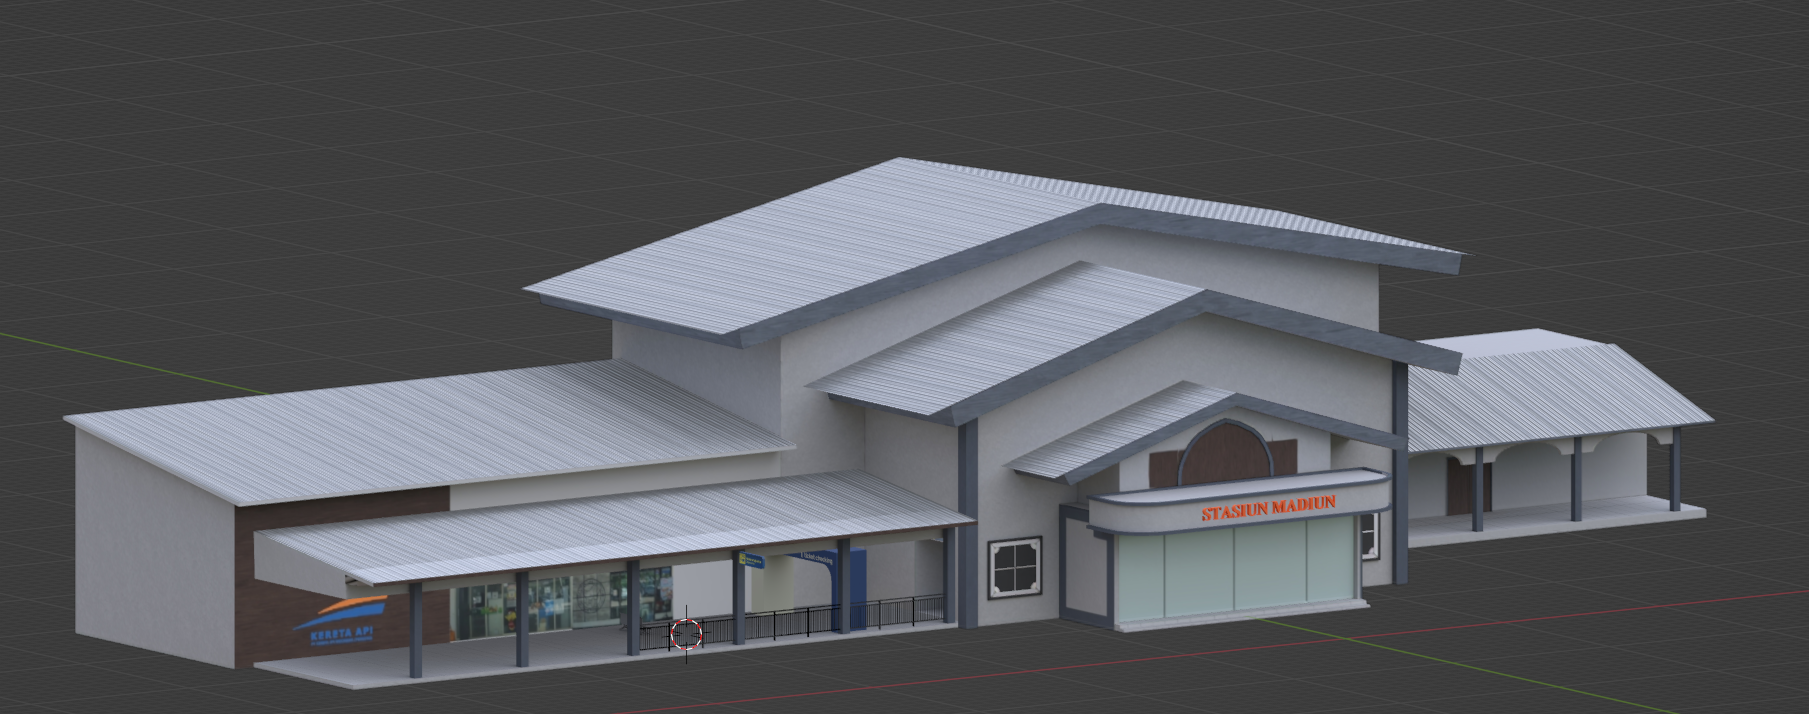
\includegraphics[width=0.6\textwidth]{resources/chapter-3-stasiun-madiun-model.png}
    \caption{Model Stasiun Madiun}
    \label{fig:stasiun-madiun-model}
\end{figure}

\begin{figure}[!h]
    \centering
    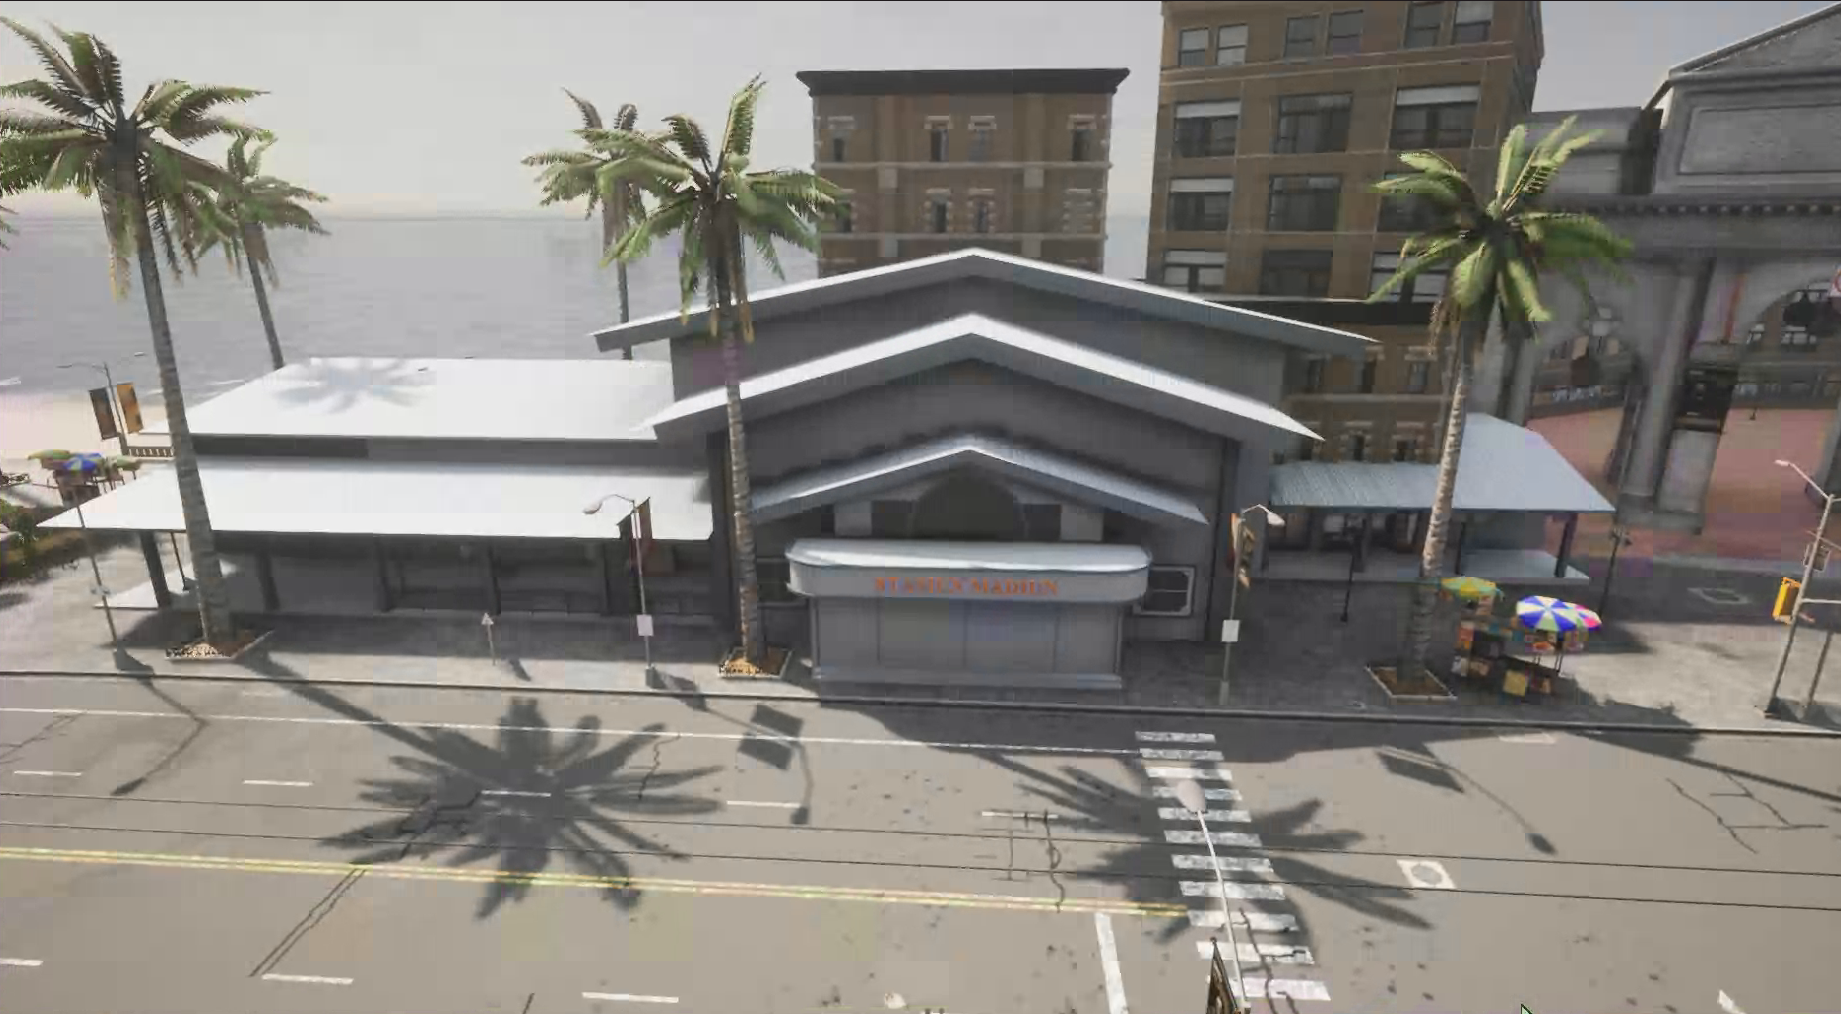
\includegraphics[width=0.6\textwidth]{resources/chapter-4/stasiun-madiun-carla.png}
    \caption{Implementasi stasiun Madiun dalam lingkungan simulasi}
    \label{fig:stasiun-madiun}
\end{figure}

Gambar \ref{fig:stasiun-solokota-model} menunjukkan aset model 3D Stasiun
Solokota yang dibuat. Gambar \ref{fig:stasiun-solokota} menunjukkan implementasi
model Stasiun Solokota dalam lingkungan simulasi.

\begin{figure}[!h]
    \centering
    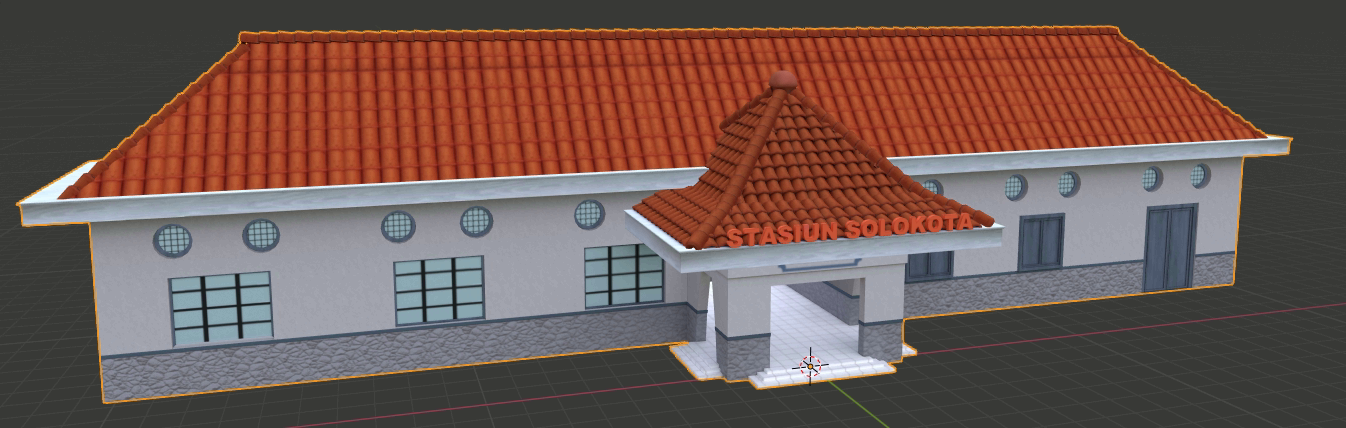
\includegraphics[width=0.6\textwidth]{resources/chapter-3-stasiun-solokota-model.png}
    \caption{Model Stasiun Solokota}
    \label{fig:stasiun-solokota-model}
\end{figure}

\begin{figure}[!h]
    \centering
    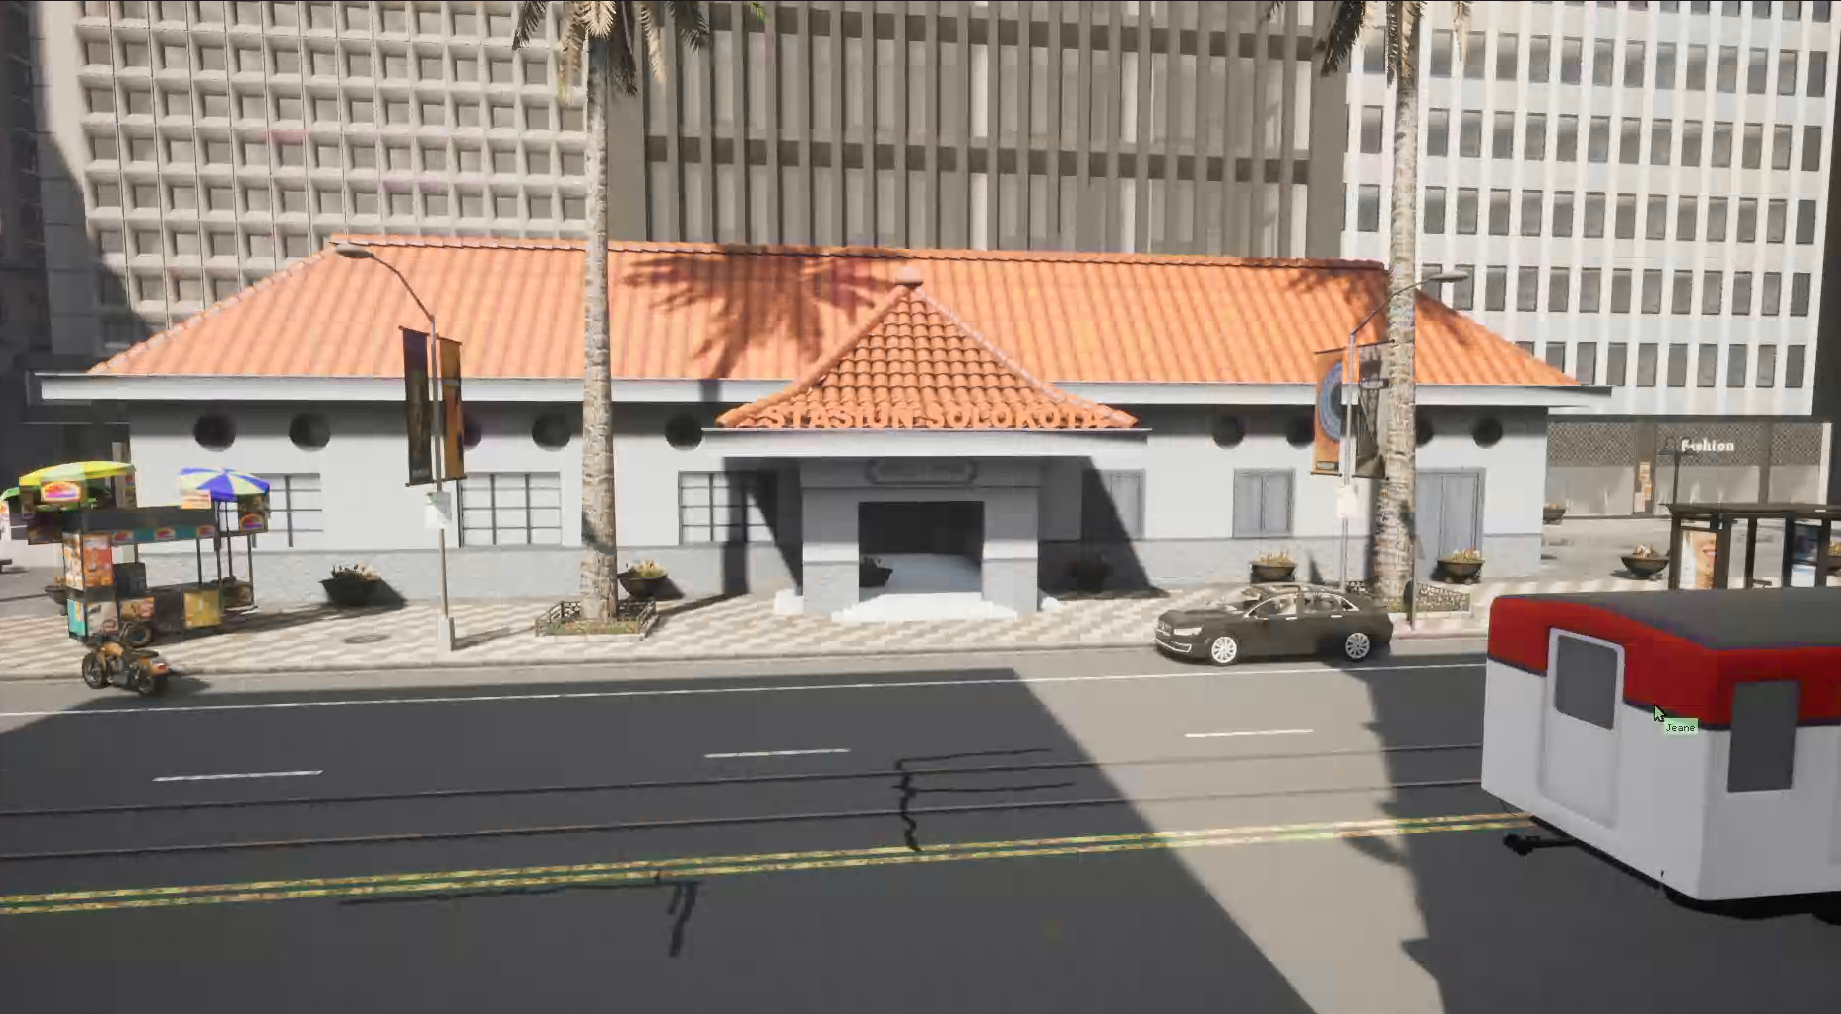
\includegraphics[width=0.6\textwidth]{resources/chapter-4/stasiun-solokota-carla.png}
    \caption{Implementasi stasiun Solokota dalam lingkungan simulasi}
    \label{fig:stasiun-solokota}
\end{figure}

Gambar \ref{fig:road-signs} menunjukkan implementasi rambu-rambu lalu lintas
dalam lingkungan simulasi.

\begin{figure}[!h]
    \centering
    \subfloat[]{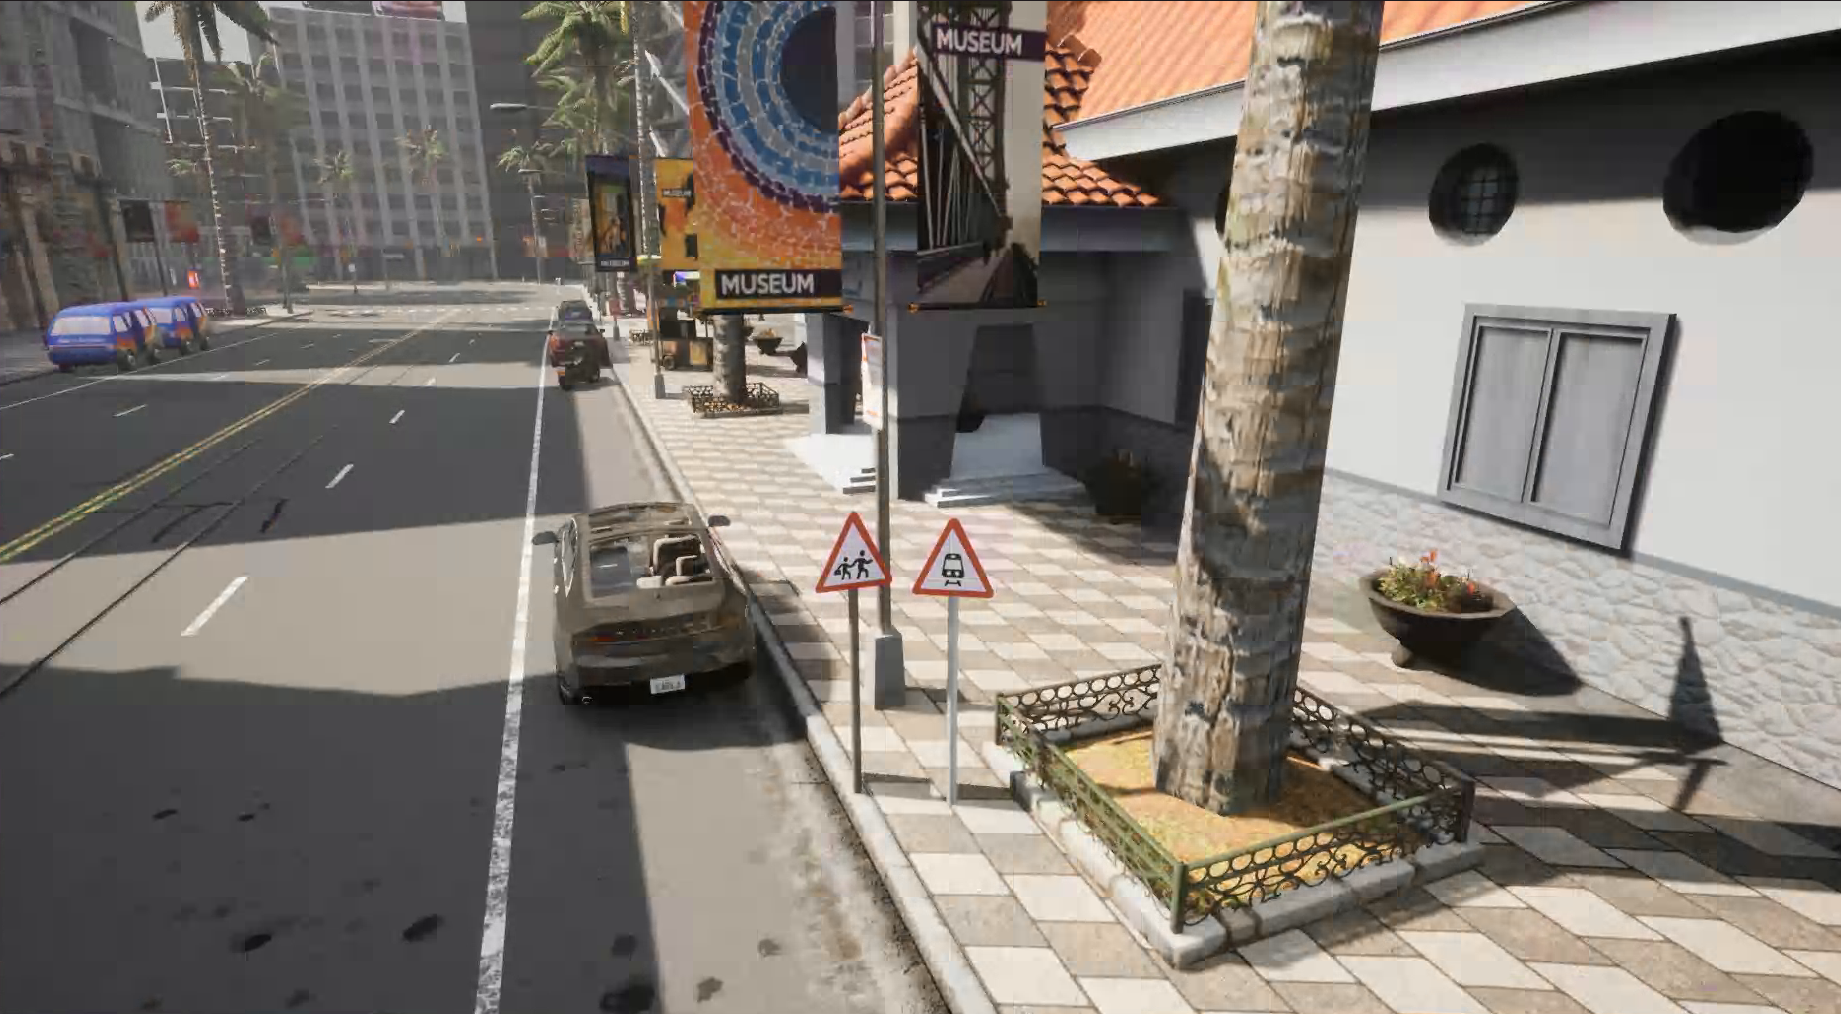
\includegraphics[width=0.45\textwidth]{resources/chapter-4/rambu-1.png}}
    \hfill
    \subfloat[]{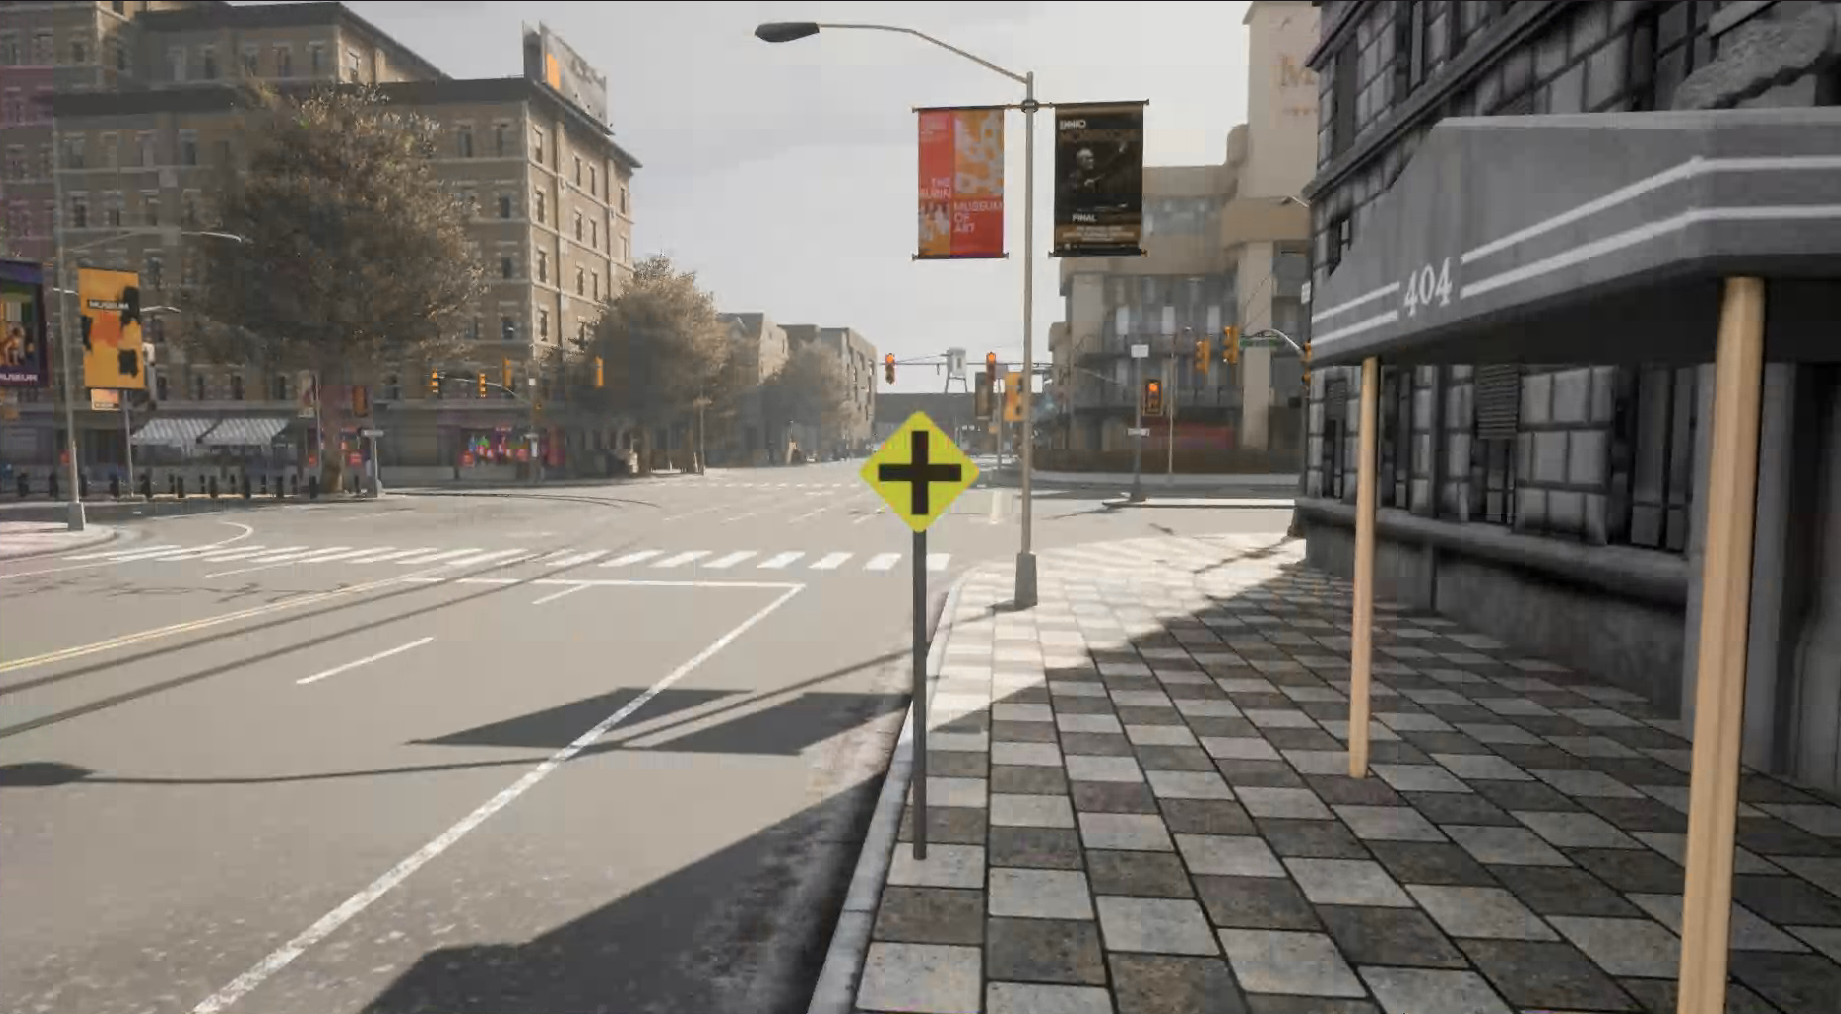
\includegraphics[width=0.45\textwidth]{resources/chapter-4/rambu-2.png}}
    \caption{Implementasi rambu-rambu lalu lintas dalam lingkungan simulasi}
    \label{fig:road-signs}
\end{figure}

\subsubsection{Rel}

Rel diimplementasi dengan menggunakan \textit{blueprint} \verb|BP_Spline| yang
terdapat pada direktori \verb|/Content/Carla/Blueprints/LevelDesign/|.
\verb|BP_Spline| merupakan \textit{blueprint} yang dapat digunakan untuk
deformasi \textit{mesh} sehingga \textit{mesh} dapat membentuk atau mengikuti
garis/kurva. Karena \verb|BP_Spline| direpresentasikan menggunakan kurva Bézier,
aset model 3D yang digunakan sebagai \textit{static mesh} harus memiliki banyak
titik sehingga dapat membentuk kurva yang mulus. Gambar \ref{fig:rel-mesh}
menunjukkan mesh aset model 3D rel yang memiliki banyak titik.

\begin{figure}[!h]
    \centering
    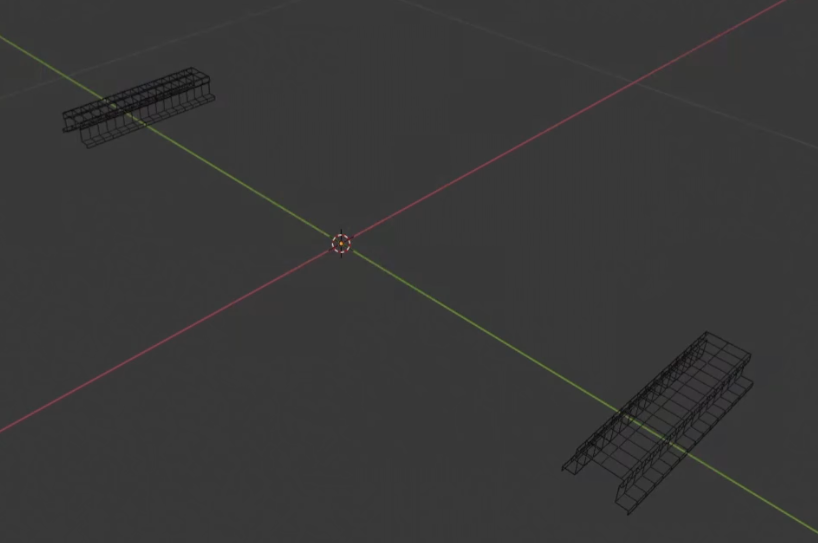
\includegraphics[width=0.5\textwidth]{resources/chapter-4/rel-mesh.png}
    \caption{Tampilan \textit{wireframe} aset model 3D rel}
    \label{fig:rel-mesh}
\end{figure}

Gambar \ref{fig:rel-route} menunjukkan 2 rute rel yang dibuat menggunakan
\textit{blueprint} \verb|BP_Spline| pada \textit{Viewport} editor.
\textit{Spline} merupakan kurva warna putih yang memiliki titik-titik dalam
bentuk kotak putih. Gambar \ref{fig:rel} menunjukkan hasil implementasi rel
dalam simulasi.

\begin{figure}[!h]
    \centering
    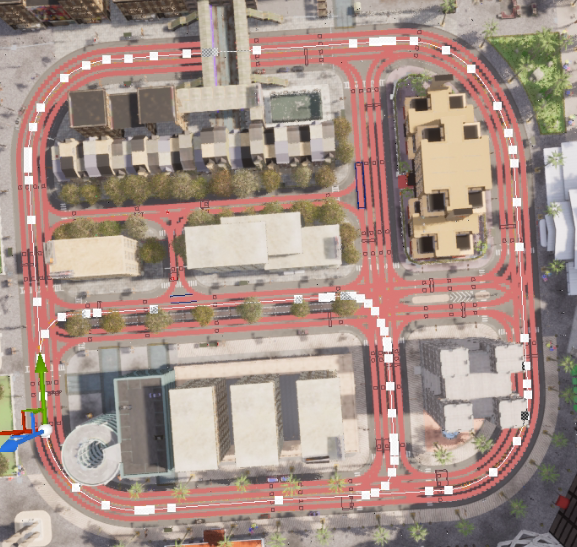
\includegraphics[width=0.47\textwidth]{resources/chapter-4/rel-route.png}
    \caption{Rute rel}
    \label{fig:rel-route}
\end{figure}

\begin{figure}[!h]
    \centering
    \subfloat[Tampilan biasa]{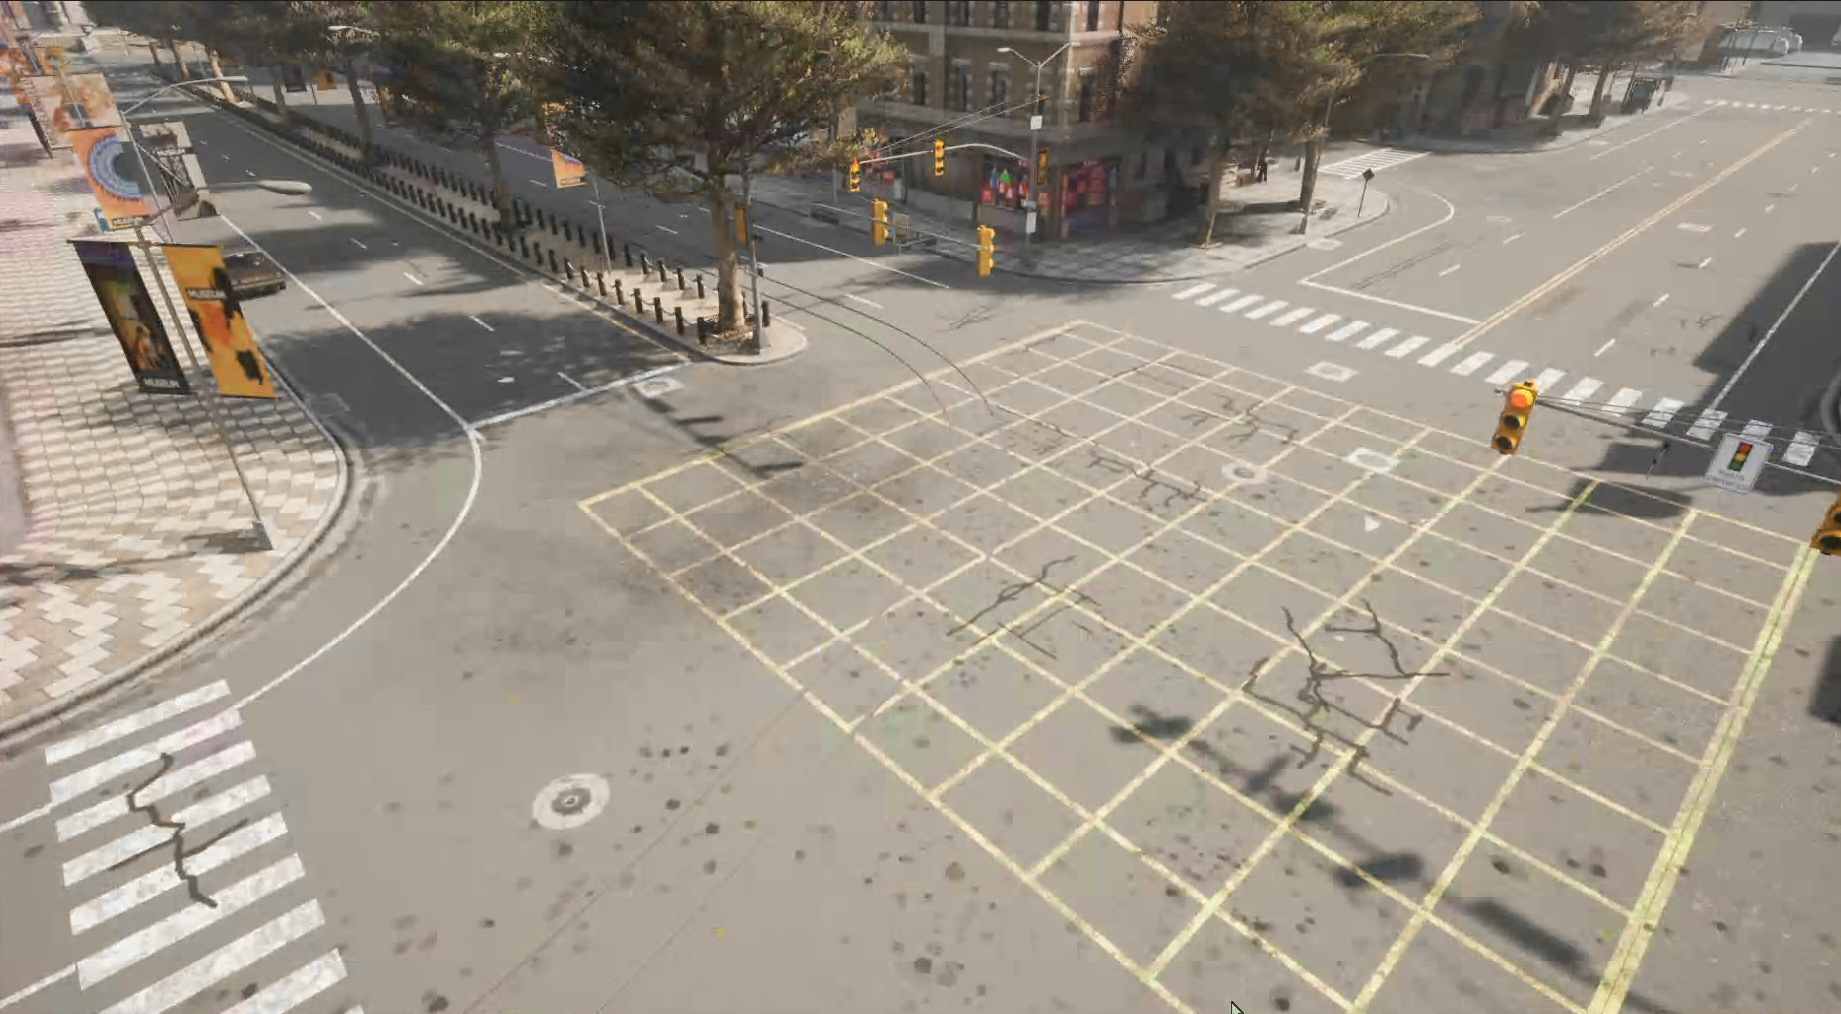
\includegraphics[width=0.47\textwidth]{resources/chapter-4/rel.png}}
    \hfill
    \subfloat[Tampilan segmentasi semantik]{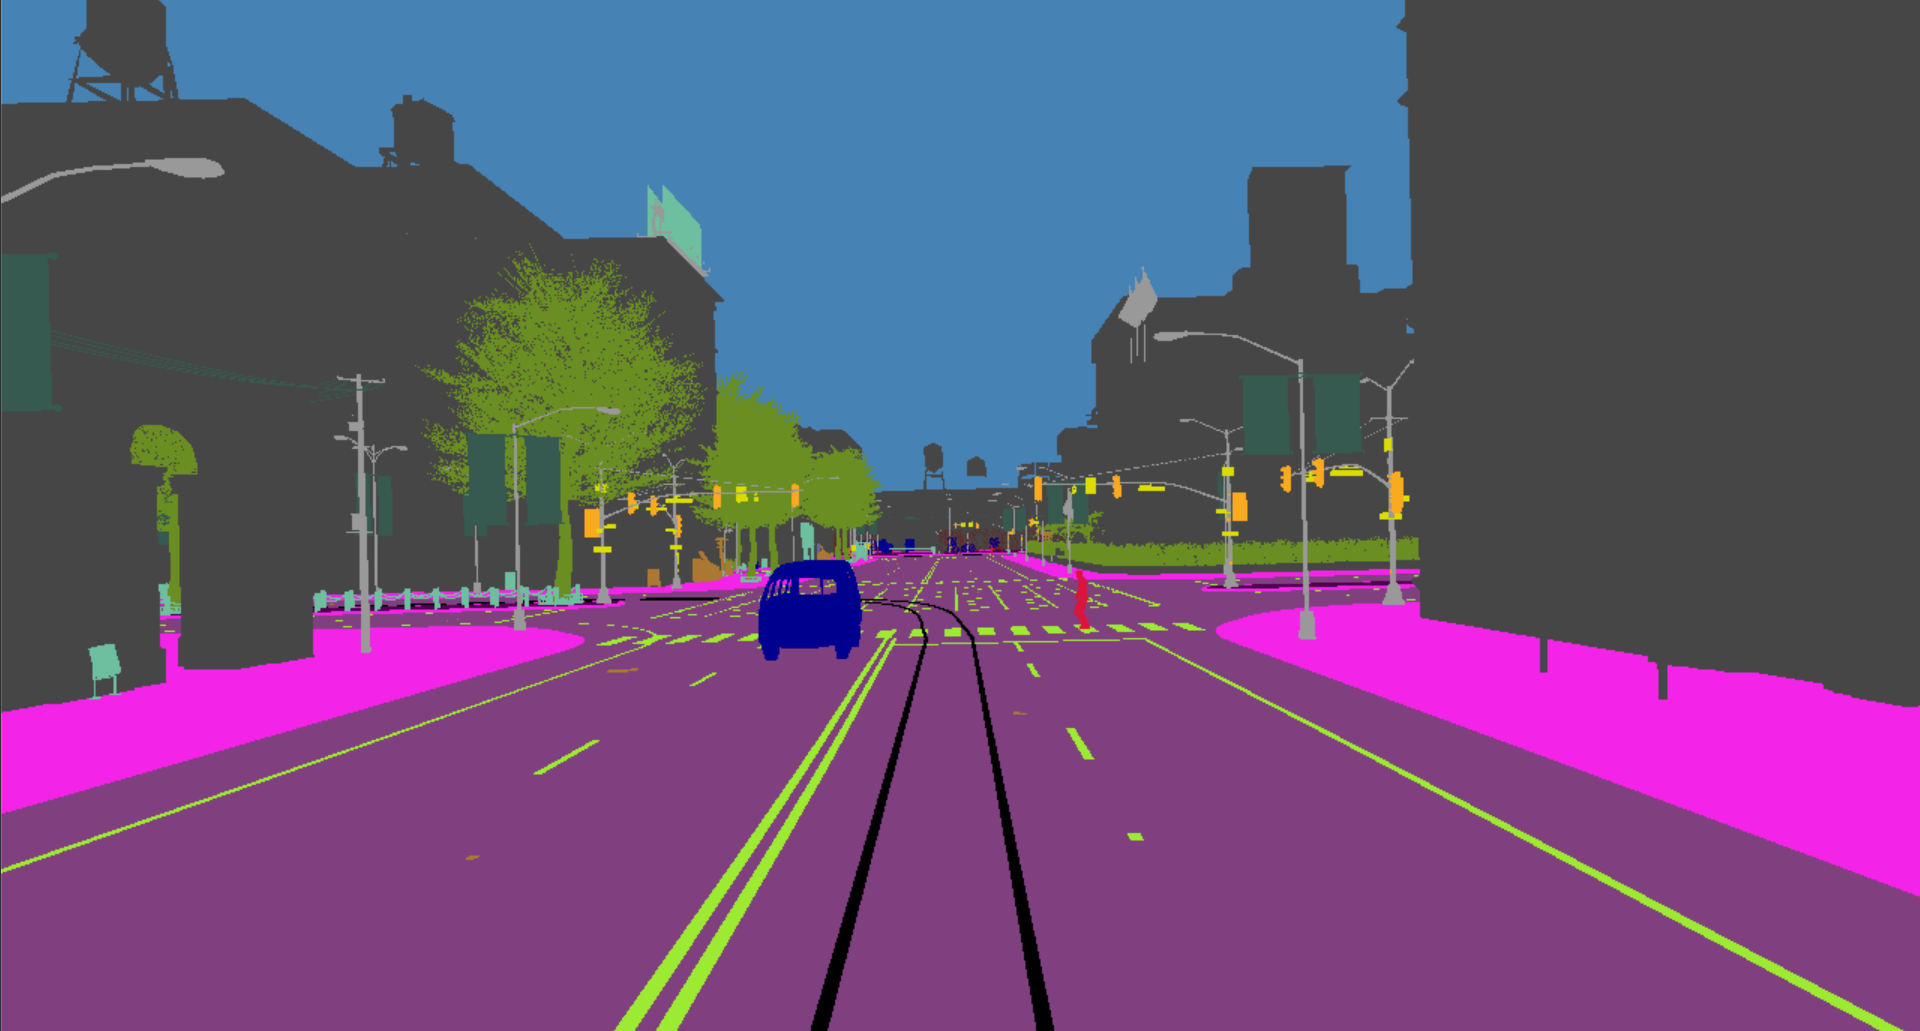
\includegraphics[width=0.47\textwidth]{resources/chapter-4/rel-segmentation-camera.png}}
    \caption{Implementasi rel dalam lingkungan simulasi}
    \label{fig:rel}
\end{figure}

\section{Validasi}

Subbab ini membahas mengenai tujuan validasi, metode validasi, dan hasil
validasi dari hasil implementasi yang telah dilakukan.

\subsection{Tujuan Validasi}

Validasi hasil dilakukan terhadap hasil implementasi objek-objek non-statik atau
objek yang dapat bergerak, yaitu objek-objek kendaraan. Objek statik yang telah
diimplementasi tidak perlu divalidasi karena objek statik tidak akan berubah
selama simulasi berjalan. Berikut adalah tujuan validasi yang ingin dicapai:

\begin{enumerate}
    \item Kendaraan stabil saat simulasi berjalan dan tidak berperilaku di luar
    harapan
    % \item Kendaraan berperilaku normal seperti kendaraan aslinya
    \item Kendaraan dapat mengikuti kendali yang diberikan pengguna
    \item Kendaraan berjalan dengan baik ketika dikendalikan secara
    \textit{autopilot}
\end{enumerate}

\subsection{Metode Validasi}

Validasi dilakukan dengan menjalankan simulasi dan melakukan 3 hal sebagai
berikut:

\begin{enumerate}

    \item Menjalankan perintah \verb|python3 manual_control.py --filter|
    \verb|<nama_kendaraan>| dalam direktori \verb|/PythonAPI/examples/| pada
    terminal untuk menguji kendali kendaraan secara manual untuk
    \textit{throttle}, \textit{brake}, dan \textit{steer}

    \item Menjalankan perintah \verb|python3 generate_traffic.py --filterv|
    \verb|<nama_kendaraan> -n <jumlah_kendaraan> -w 0| dalam direktori \verb|/PythonAPI/examples/|
    pada terminal untuk menguji kendali kendaraan secara \textit{autopilot}

    Opsi \verb|-n <jumlah_kendaraan>| digunakan untuk melakukan \textit{spawn}
    kendaraan sebanyak \verb|<jumlah_kendaraan>|. Opsi \verb|-w| digunakan untuk
    melakukan \textit{spawn} \textit{walker} atau pedestrian sebanyak 0.

    \item Mengamati perilaku kendaraan saat simulasi berjalan untuk memastikan
    kendaraan stabil saat simulasi dan tidak berperilaku di luar harapan

\end{enumerate}

\subsection{Hasil Validasi}

% note: add preamble again?

\subsubsection{Validasi Trem dan Angkot}

Hasil validasi trem adalah trem dapat mengikuti kendali pengguna dan kendali
secara \textit{autopilot} dengan baik. Trem beroperasi dengan stabil dan tidak
melakukan hal yang tidak terduga selama simulasi berjalan. Gambar
\ref{fig:tram-validation} menunjukkan hasil validasi trem.

\begin{figure}[!h]
    \centering
    \subfloat[Kendali manual]{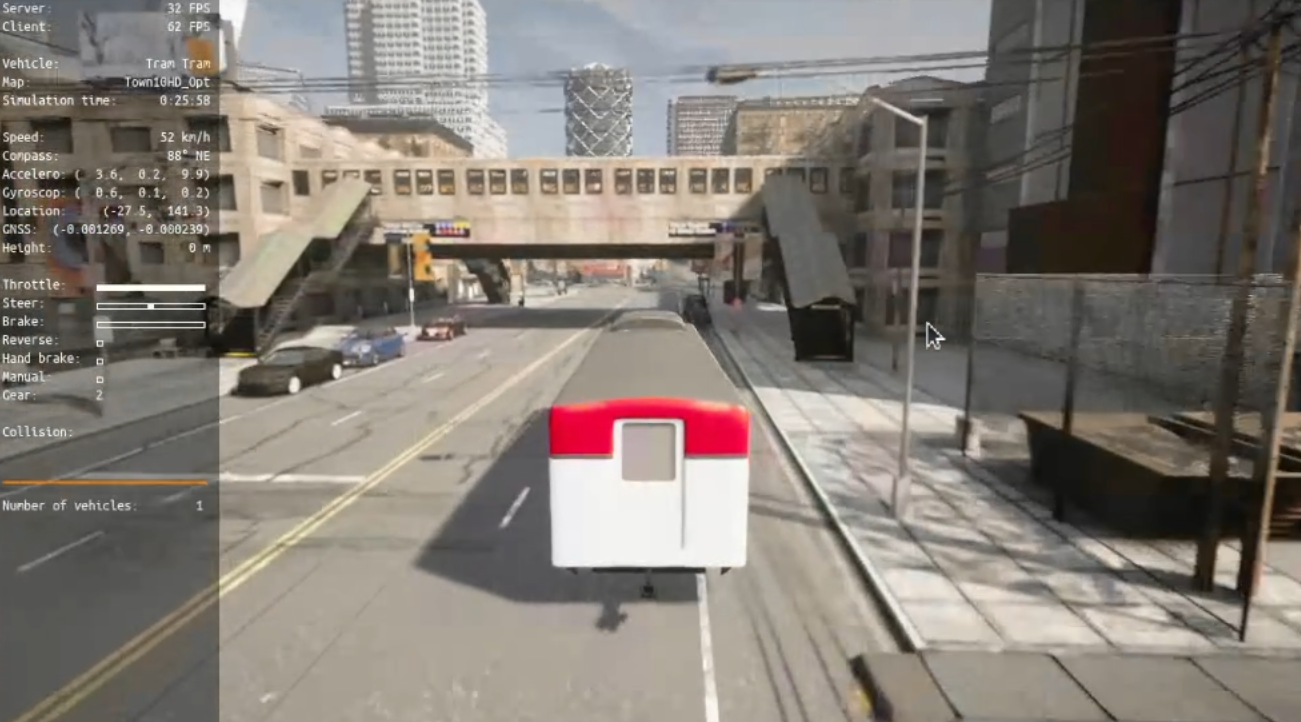
\includegraphics[width=0.47\textwidth]{resources/chapter-4/testing-tram-manual.png}}
    \hfill
    \subfloat[Kendali \textit{autopilot}]{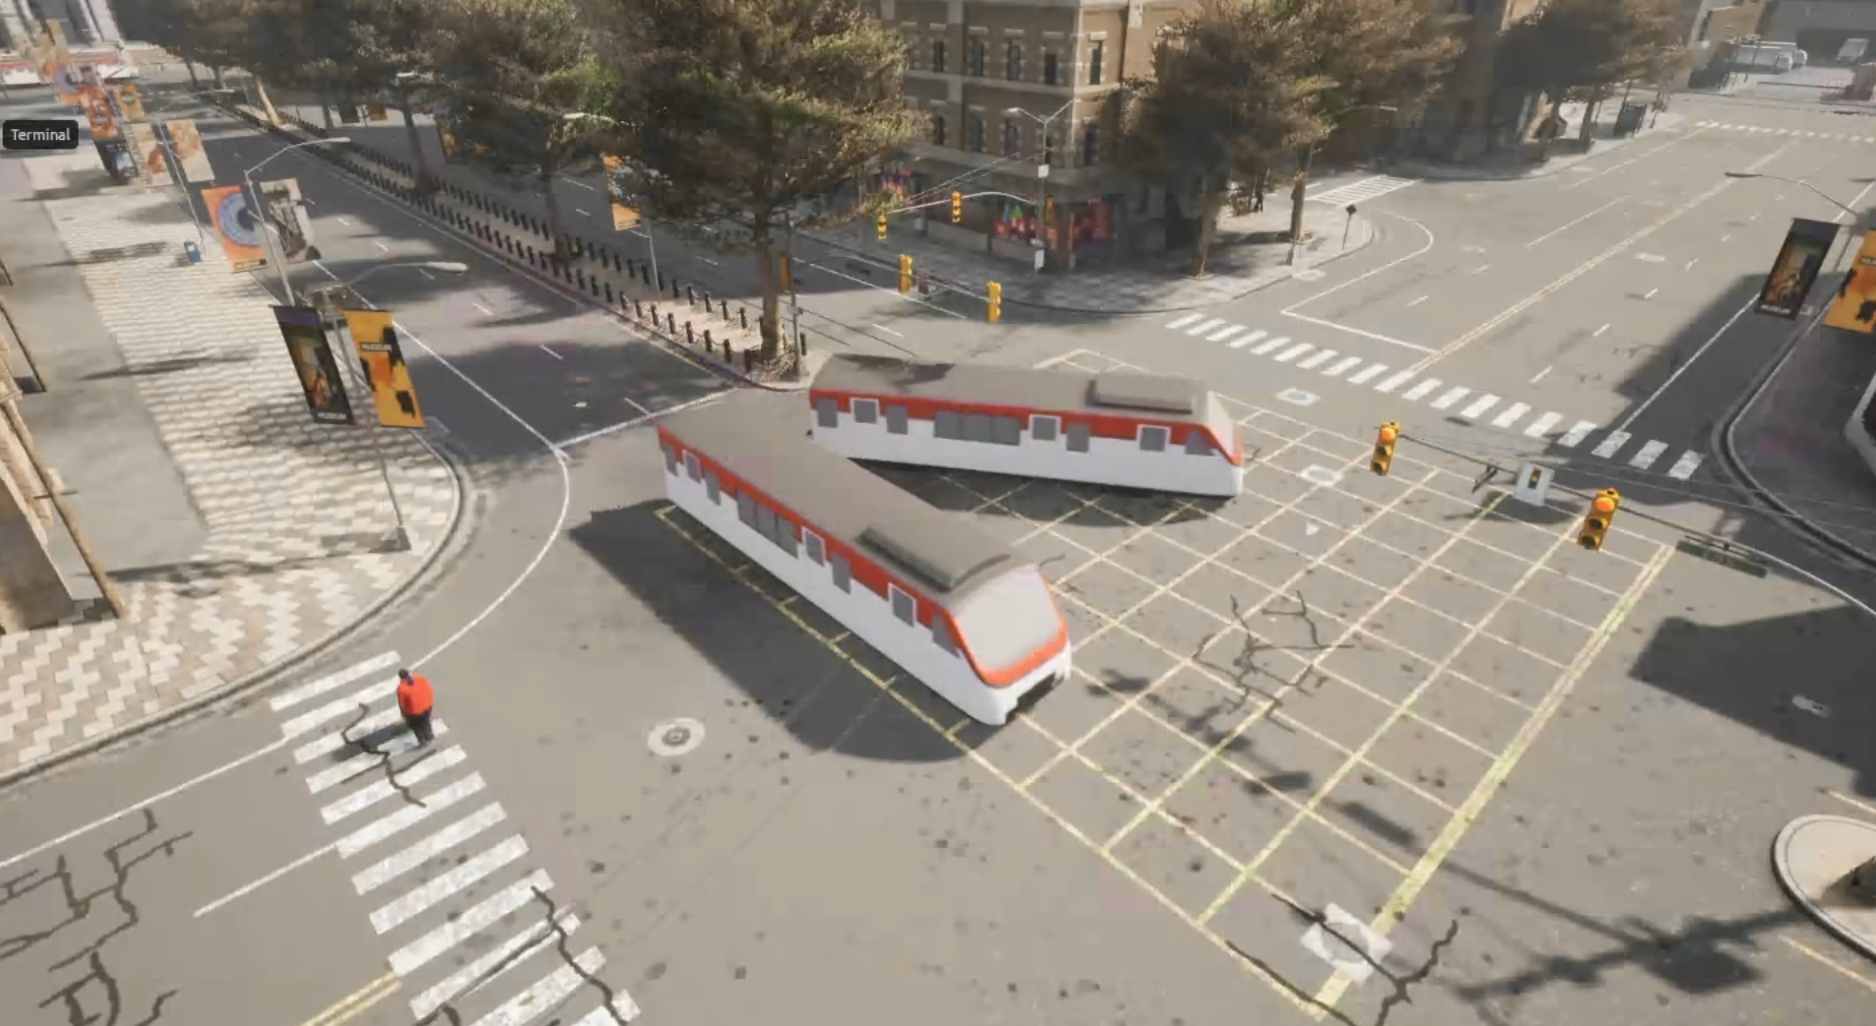
\includegraphics[width=0.47\textwidth]{resources/chapter-4/testing-tram-generate.png}}
    \caption{Validasi trem}
    \label{fig:tram-validation}
\end{figure}

Hasil validasi angkot adalah angkot dapat mengikuti kendali pengguna dan kendali
secara \textit{autopilot} dengan baik. Angkot beroperasi dengan stabil dan tidak
melakukan hal yang tidak terduga selama simulasi berjalan. Gambar
\ref{fig:angkot-validation} menunjukkan hasil validasi angkot.

\begin{figure}[!h]
    \centering
    \subfloat[Kendali manual]{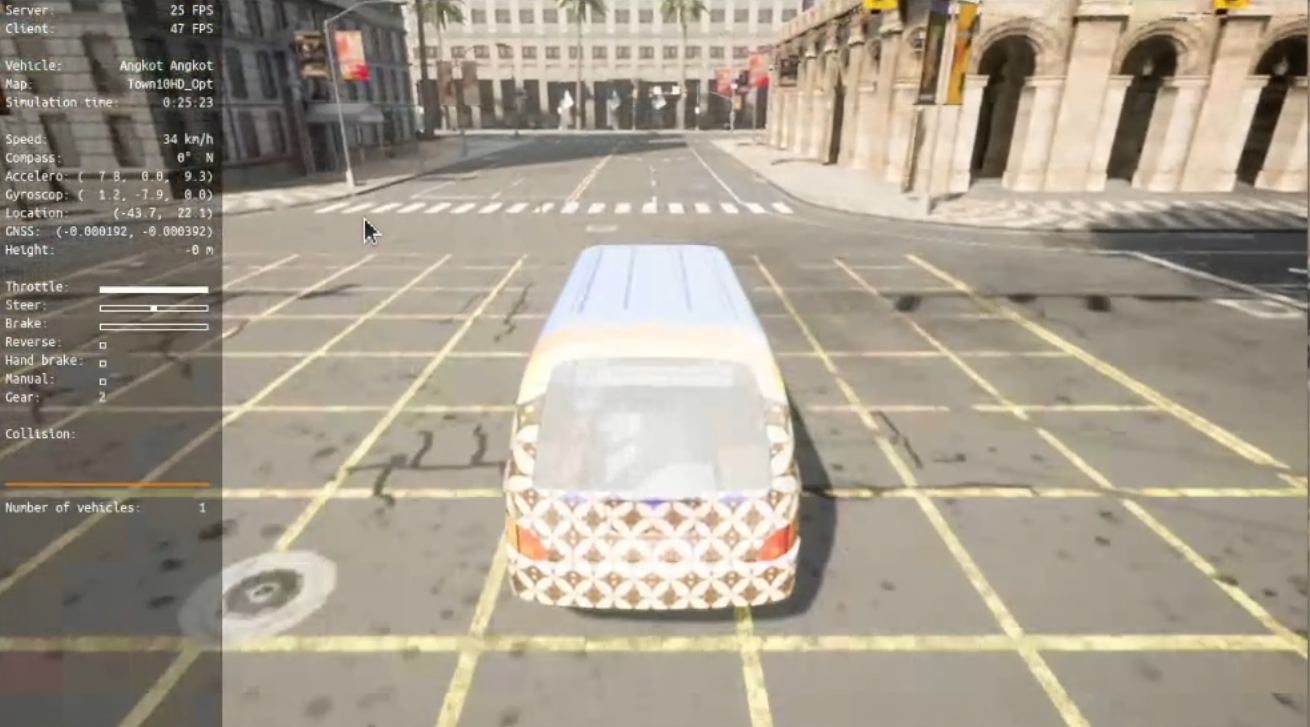
\includegraphics[width=0.47\textwidth]{resources/chapter-4/testing-angkot-manual.png}}
    \hfill
    \subfloat[Kendali \textit{autopilot}]{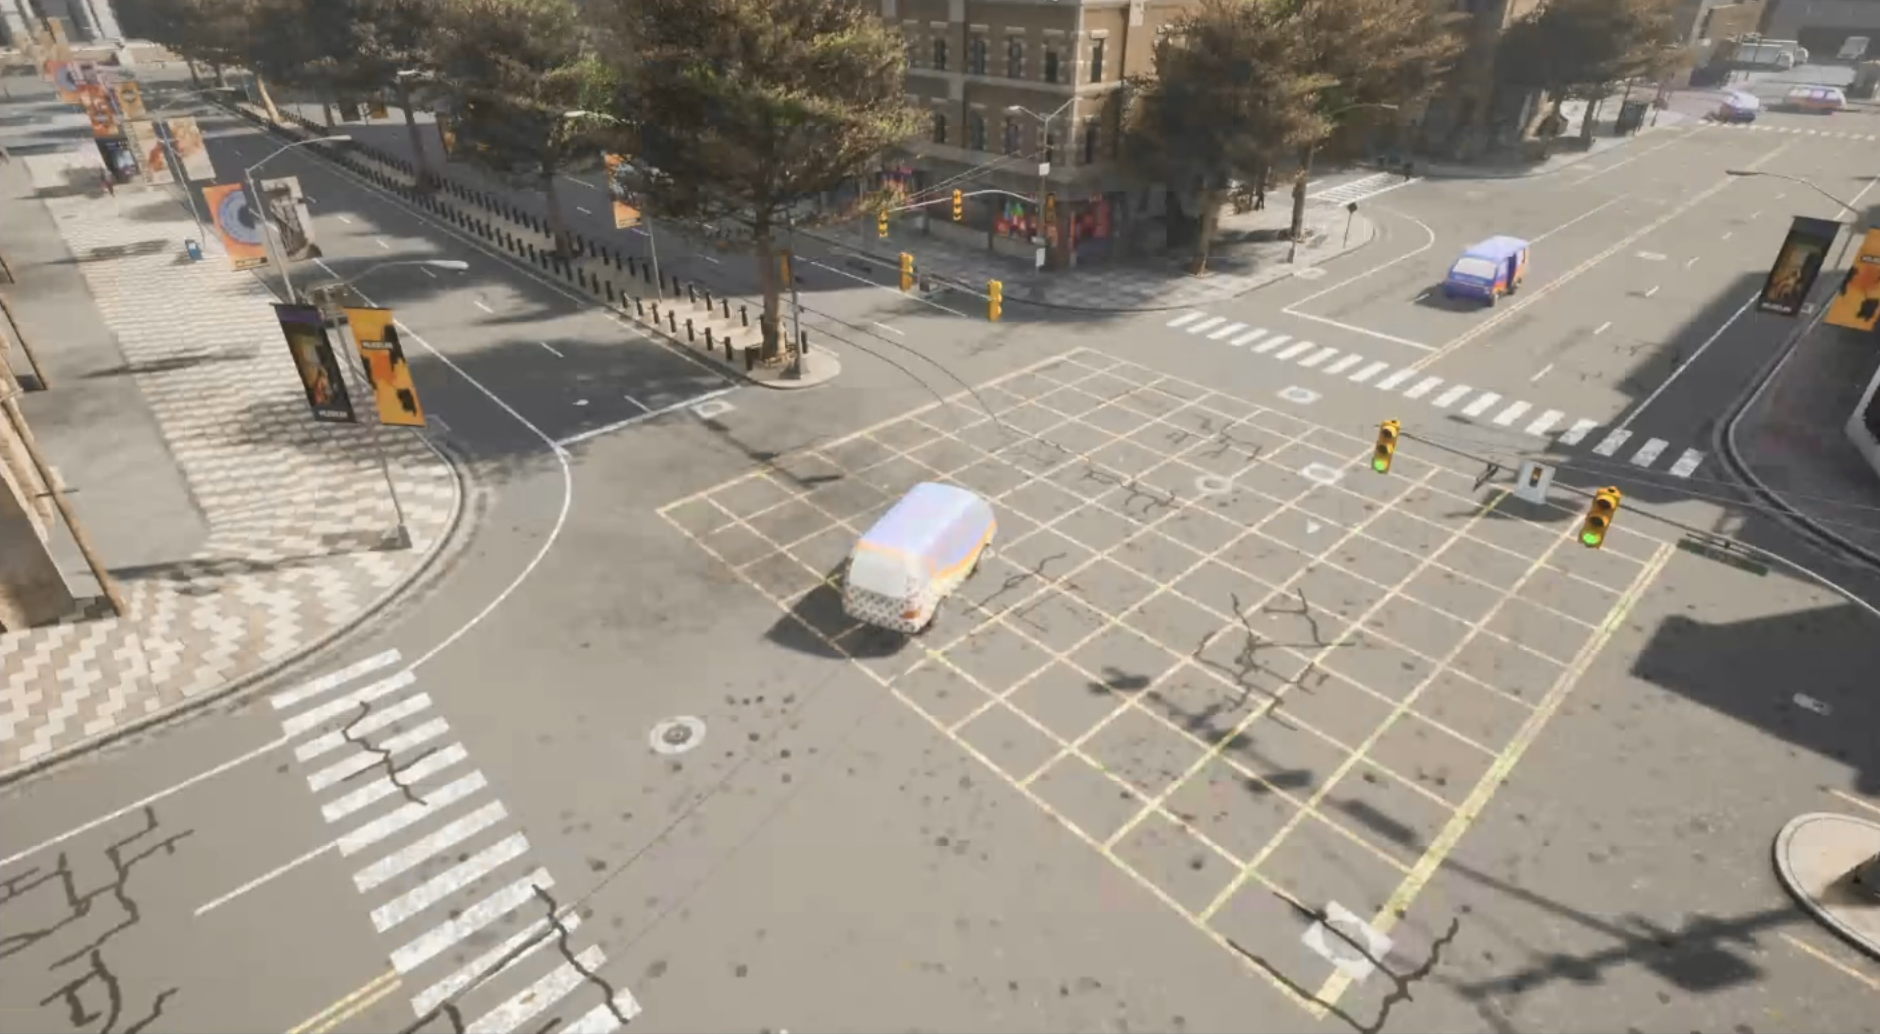
\includegraphics[width=0.47\textwidth]{resources/chapter-4/testing-angkot-generate.png}}
    \caption{Validasi angkot}
    \label{fig:angkot-validation}
\end{figure}

\subsubsection{Validasi Sepeda Onthel, Sepeda Motor, dan Becak}

Hasil validasi sepeda onthel adalah sepeda onthel tidak dapat mengikuti kendali
pengguna maupun kendali secara \textit{autopilot}. Sepeda onthel tidak dapat
beroperasi dengan stabil selama simulasi berjalan. Sepeda onthel tampak bergerak
sendiri ketika tidak ada perintah kendali dari pengguna. Ketika sepeda onthel
dikendalikan secara \textit{autopilot}, sepeda onthel bergerak secara acak
ditempat padahal seharusnya mengikuti rute yang telah ditentukan. Gambar
\ref{fig:onthel-validation} menunjukkan hasil validasi sepeda onthel yang gagal.

\begin{figure}[!h]
    \centering
    \subfloat[Kendali manual]{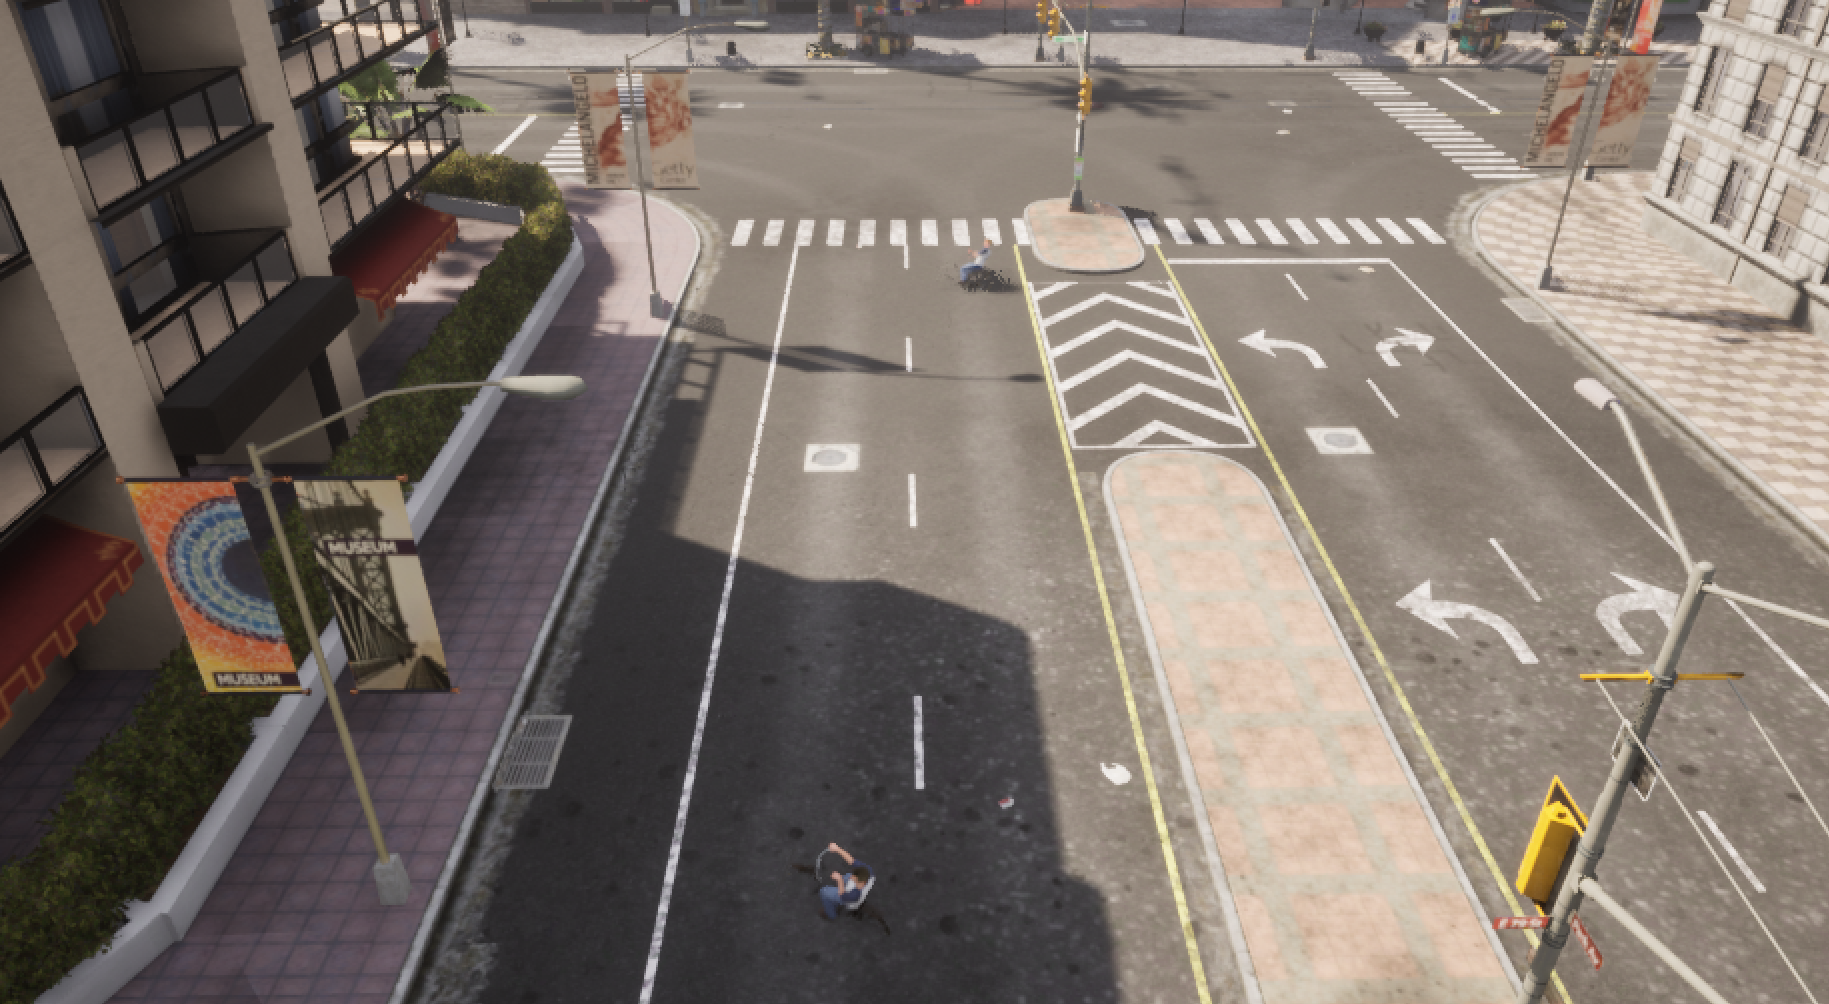
\includegraphics[width=0.47\textwidth]{resources/chapter-4/testing-onthel-generate.png}}
    \hfill
    \subfloat[Kendali \textit{autopilot}]{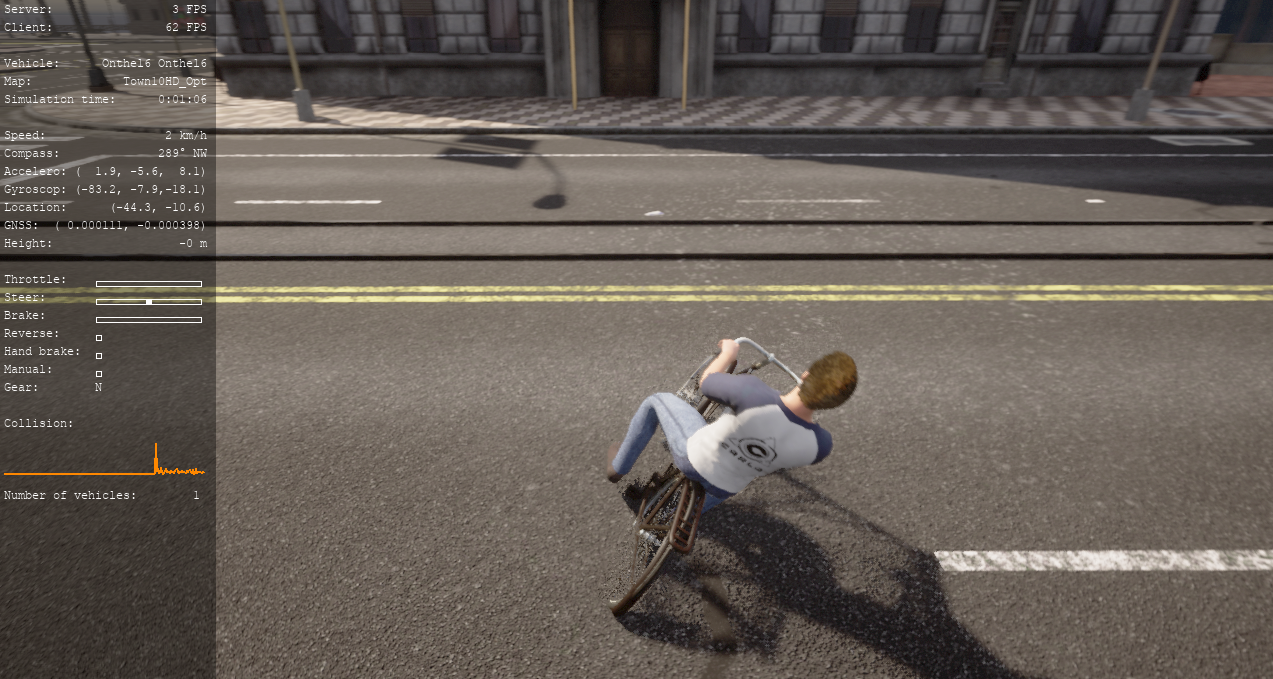
\includegraphics[width=0.47\textwidth]{resources/chapter-4/testing-onthel-manual.png}}
    \caption{Validasi sepeda onthel}
    \label{fig:onthel-validation}
\end{figure}

Karena validasi implementasi sepeda onthel tidak berhasil, sepeda motor dan
becak tidak diimplementasikan sebagai kendaraan. Gambar
\ref{fig:becak-validation} menunjukkan hasil validasi becak menggunakan kendali
\textit{autopilot} yang tidak berhasil.

\begin{figure}[!h]
    \centering
    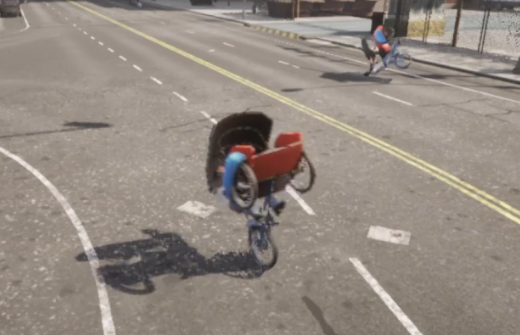
\includegraphics[width=0.5\textwidth]{resources/chapter-4/testing-becak-generate.png}
    \caption{Validasi becak}
    \label{fig:becak-validation}
\end{figure}

\section{Evaluasi}

Berdasarkan hasil validasi hasil implementasi trem dan angkot sebagai kendaraan
roda 2, implementasi trem dan angkot berhasil. Trem dan angkot dapat mengikuti
kendali pengguna dan kendali secara \textit{autopilot} dengan baik.

Hasil implementasi sepeda onthel, sepeda motor, dan becak sebagai kendaraan roda
2 tidak stabil berdasarkan hasil validasi. Kendaraan-kendaraan roda 2 tersebut
tidak dapat mengikuti kendali pengguna maupun kendali secara \textit{autopilot},
kendaraan terlihat bergerak ketika seharusnya diam, dan roda kendaraan terlihat
tenggelam menembus jalan. Ketidakstabilan tersebut diakibatkan oleh implementasi
yang kurang sempurna. Implementasi kurang sempurna disebabkan oleh implementasi
dilakukan mengikuti dokumentasi yang kurang lengkap. Hasil implementasi yang
stabil dipersulit juga oleh editor CARLAUE4 yang sering \textit{crash} jika
sedang mengedit kendaraan roda 2. Kejadian \textit{crash} dari editor
kemungkinan besar terjadi disebabkan oleh adanya \textit{error} dari aplikasi
dan bukan disebabkan oleh sumber daya perangkat keras. Hal tersebut terbukti
ketika editor juga mengalami \textit{crash} ketika digunakan di komputer SILS
(komputer bersama yang digunakan). Komputer tersebut memiliki spesifikasi yang
melebihi dari spesifikasi yang direkomendasikan oleh CARLA.

Implementasi kendaraan roda 2 dilakukan berulang-ulang untuk mencoba mengatasi
kekuranglengkapan dokumentasi. Implementasi kendaraan roda 2 yang dilakukan
berulang dengan mengubah hal-hal yang memungkinkan kesalahan implementasi atau
dengan cara \textit{trial-and-error} namun tidak berhasil. Kemungkinan kesalahan
implementasi terletak pada proses \textit{skinning} karena kekuranglengkapan
dokumentasi dalam penjelasan bagian apa saja yang harus dihubungkan dengan
kerangka atau \textit{armature} yang disediakan. Selain itu, implementasi juga
mungkin terganggu oleh dokumentasi yang tidak diperbarui atau tidak sesuai
dengan editor.

Adanya keterbatasan lain dari CARLA yaitu tidak dapat mengimplementasikan
kendaraan roda ganjil ataupun sejumlah \textit{n}. Becak seharus diimplementasi
sebagai kendaraan roda 3 namun kendaraan roda 3 tidak dapat diimplementasikan
menggunakan CARLA versi 0.9.12. maupun versi 0.9.13.

Sepeda onthel, sepeda motor, dan becak tidak diimplementasikan sebagai kendaraan
roda 2 karena hasil validasi tidak stabil. Oleh karena itu, kendaraan-kendaraan
tersebut diimplementasikan sebagai objek statis.

\section{Distribusi Hasil Implementasi}

Setelah semua objek lokal dan lingkungan simulasi selesai dibuat, aset yang
telah divalidasi didistribusikan dalam bentuk CARLA versi \textit{packaged}.
CARLA versi \textit{packaged} tersebut dibuat dengan cara menjalankan perintah
\verb|make package| pada terminal. Perintah tersebut menghasilkan 2 hal dalam
direktori \verb|/Dist/|, yaitu sebuah \textit{folder}
\verb|CARLA_Shipping_0.9.12| dan berkas \verb|CARLA_0.9.12.tar.gz|.
\textit{Folder} \verb|CARLA_Shipping_0.9.12| berisi CARLA yang memiliki
aset-aset baru, sudah di-\textit{compile}, dan siap untuk dijalankan tanpa
editor. Berkas \verb|CARLA_0.9.12.tar.gz| adalah berkas yang mengandung
aset-aset baru yang harus diimpor jika ingin digunakan.
